\begin{appendices}

\chapter{Mockups de Interfaces del Sistema}
\label{anexo:Mockups}

% ------------------------------------------------------------------------------
% SECCIÓN 1: PERFIL QUEJOSO
% ------------------------------------------------------------------------------
\section{Perfil: Quejoso}
Este perfil corresponde a la comunidad politécnica (alumnos, docentes, administrativos). Las interfaces se centran en la accesibilidad y el seguimiento simple.

% --- VISTA 01 ---
\begin{figure}[h]
    \centering
    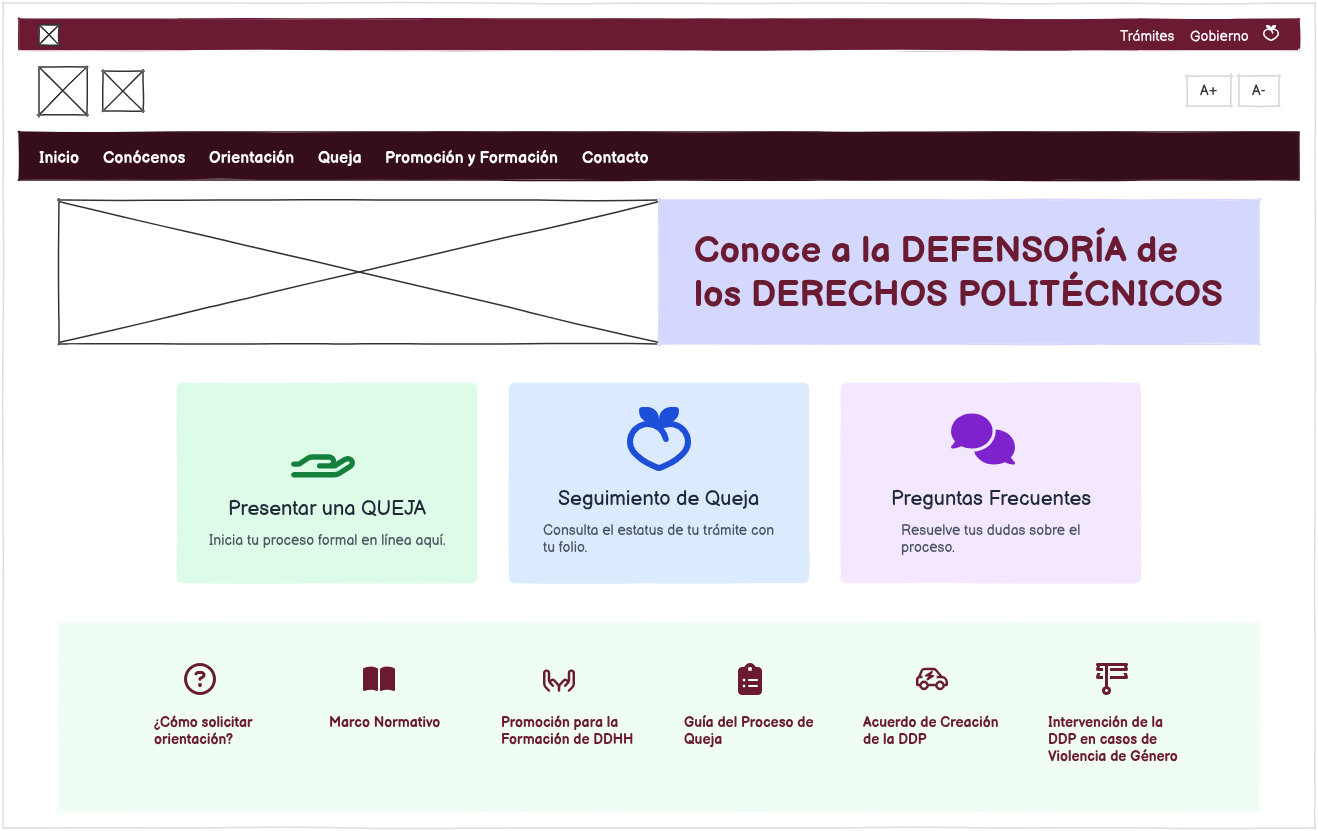
\includegraphics[width=0.9\textwidth]{imagenes/quejoso/Inicio.png}
    \caption{MQ-01: Pantalla de inicio y selección de trámite.}
    \label{fig:mq01_inicio}
\end{figure}

\noindent \textbf{Descripción de la interfaz (MQ-01):} \\
La pantalla de inicio constituye el punto de entrada principal para el usuario. Presenta una arquitectura de información clara basada en la identidad institucional del IPN. Los elementos clave incluyen:
\begin{itemize}
    \item \textbf{Menú de Navegación:} Acceso a secciones informativas como Conócenos y Marco Normativo.
    \item \textbf{Accesos Directos:} Tres contenedores principales para "Presentar una QUEJA", "Seguimiento de Queja" (mediante folio) y "Preguntas Frecuentes".
    \item \textbf{Footer Informativo:} Iconografía para acceso rápido a guías de proceso, normatividad y protocolos de violencia de género.
\end{itemize}

\vspace{1cm} % Espacio antes de la siguiente figura

% --- VISTA 02 ---
\begin{figure}[h]
    \centering
    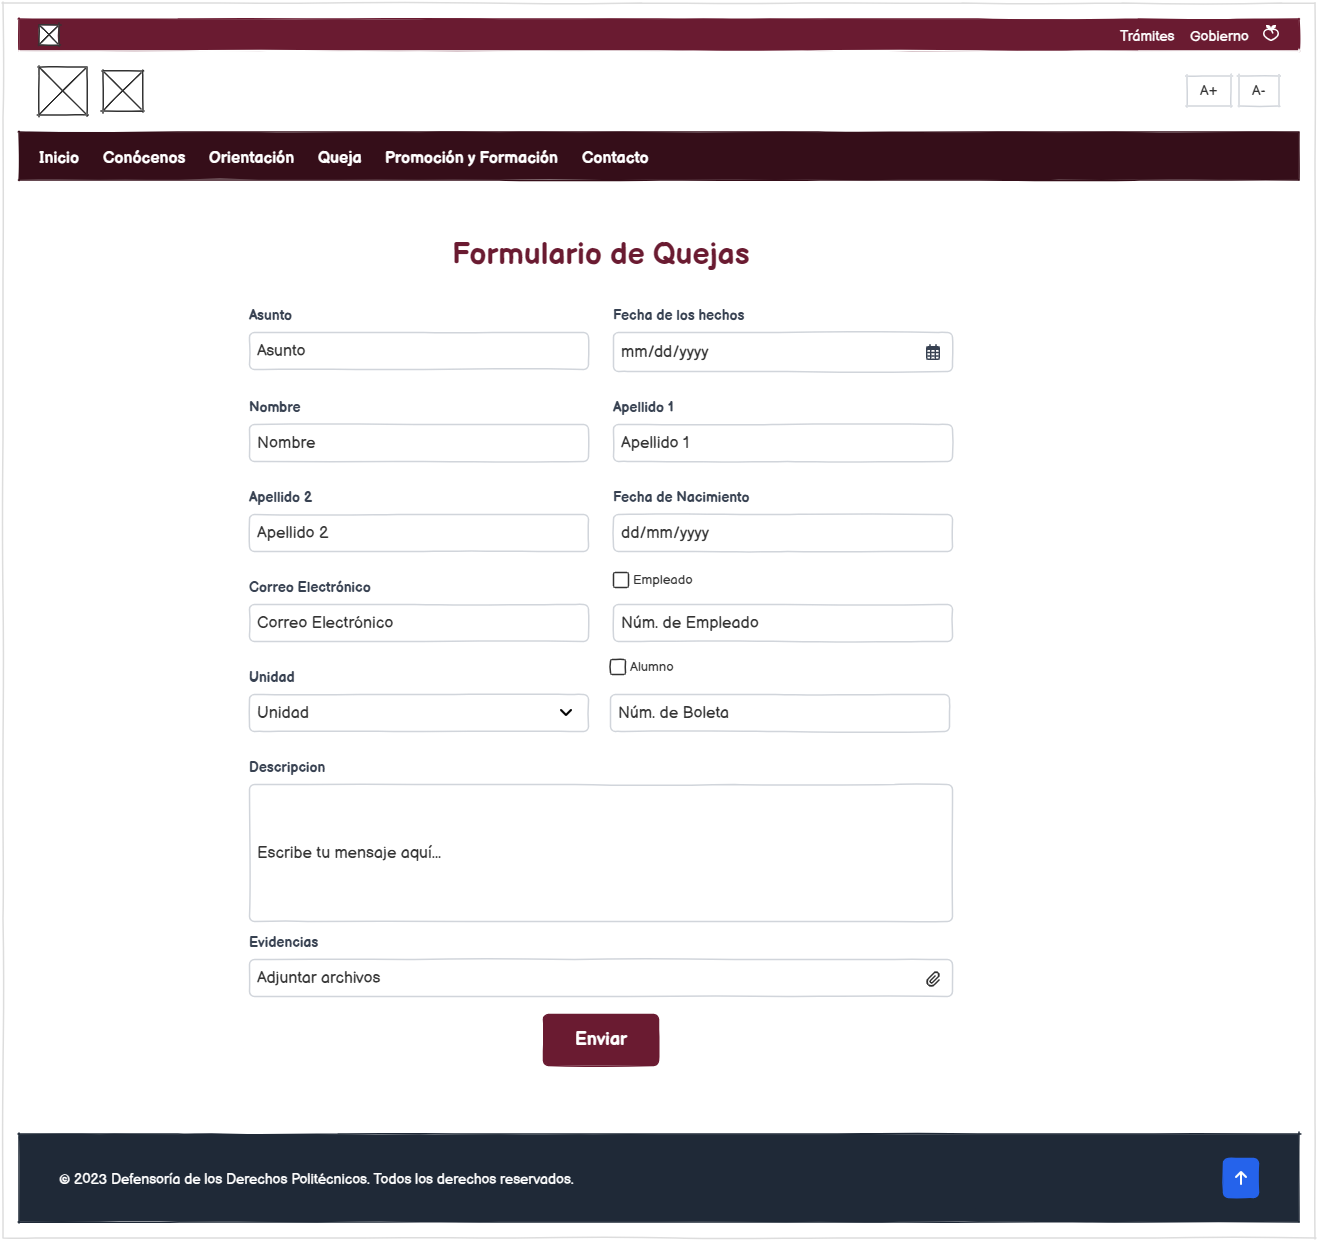
\includegraphics[width=0.85\textwidth]{imagenes/quejoso/FormularioQueja.png}
    \caption{MQ-02: Formulario para el registro de quejas.}
    \label{fig:mq02_formulario}
\end{figure}

\noindent \textbf{Descripción de la interfaz (MQ-02):} \\
Esta interfaz permite al usuario capturar los datos personales que serán utilizados por la Defensoría de Derechos Politécnicos, así como capturar la redacción del suceso. Este formulario esta compuesto por:
\begin{itemize}
    \item \textbf{Datos Generales:} Campos para el asunto, nombre completo, fecha de los hechos y fecha de nacimiento.
    \item \textbf{Identificación de Usuario:} Selección mediante \textit{checkbox} para perfil de Empleado (con número de empleado) o Alumno (con número de boleta).
    \item \textbf{Información de Contacto y Ubicación:} Campo para correo electrónico y un menú desplegable para seleccionar la Unidad Académica o Administrativa correspondiente.
    \item \textbf{Cuerpo de la Queja:} Área de texto de formato libre para la descripción de los hechos y un campo de carga de archivos para adjuntar evidencias.
    \item \textbf{Botón de Acción:} Botón prominente de enviar para procesar la información.
\end{itemize}

% --- VISTA 03 ---
\begin{figure}[h]
    \centering
    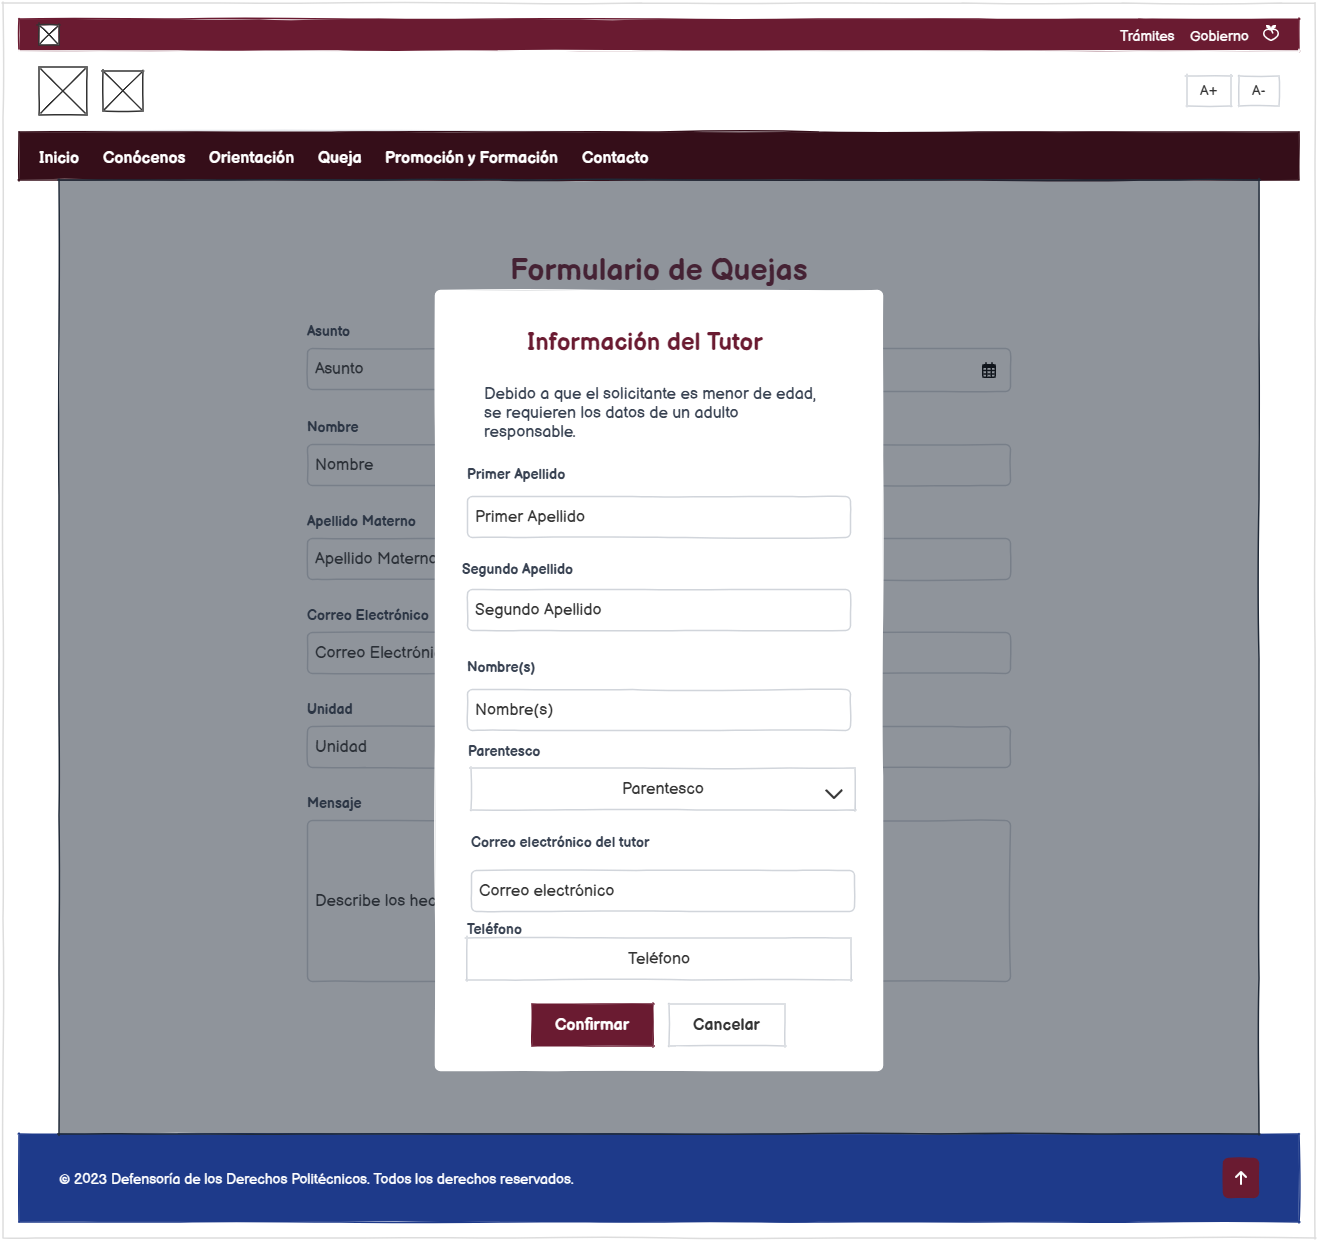
\includegraphics[width=0.85\textwidth]{imagenes/quejoso/FormularioTutor.png}
    \caption{MQ-03: Ventana emergente de información del tutor para menores de edad.}
    \label{fig:mq03_tutor}
\end{figure}

\noindent \textbf{Descripción de la interfaz (MQ-03):} \\
Esta interfaz presenta una ventana modal (emergente) que se activa automáticamente cuando el sistema detecta, mediante la fecha de nacimiento, que el solicitante es menor de edad. Sus componentes son:
\begin{itemize}
    \item \textbf{Mensaje Informativo:} Notificación clara que explica la necesidad legal de contar con los datos de un adulto responsable.
    \item \textbf{Datos del Tutor:} Campos específicos para capturar el nombre completo (apellidos y nombres) del representante legal.
    \item \textbf{Parentesco:} Menú desplegable para seleccionar la relación con el menor (padre, madre, tutor legal, etc.).
    \item \textbf{Contacto del Adulto:} Campos validados para el correo electrónico y teléfono de contacto del tutor.
    \item \textbf{Controles de Acción:} Botón de "Confirmar" para validar los datos e incorporarlos al expediente, y un botón de "Cancelar" para volver al formulario principal.
\end{itemize}

\vspace{1cm}

% --- VISTA 04 ---
\begin{figure}[h]
    \centering
    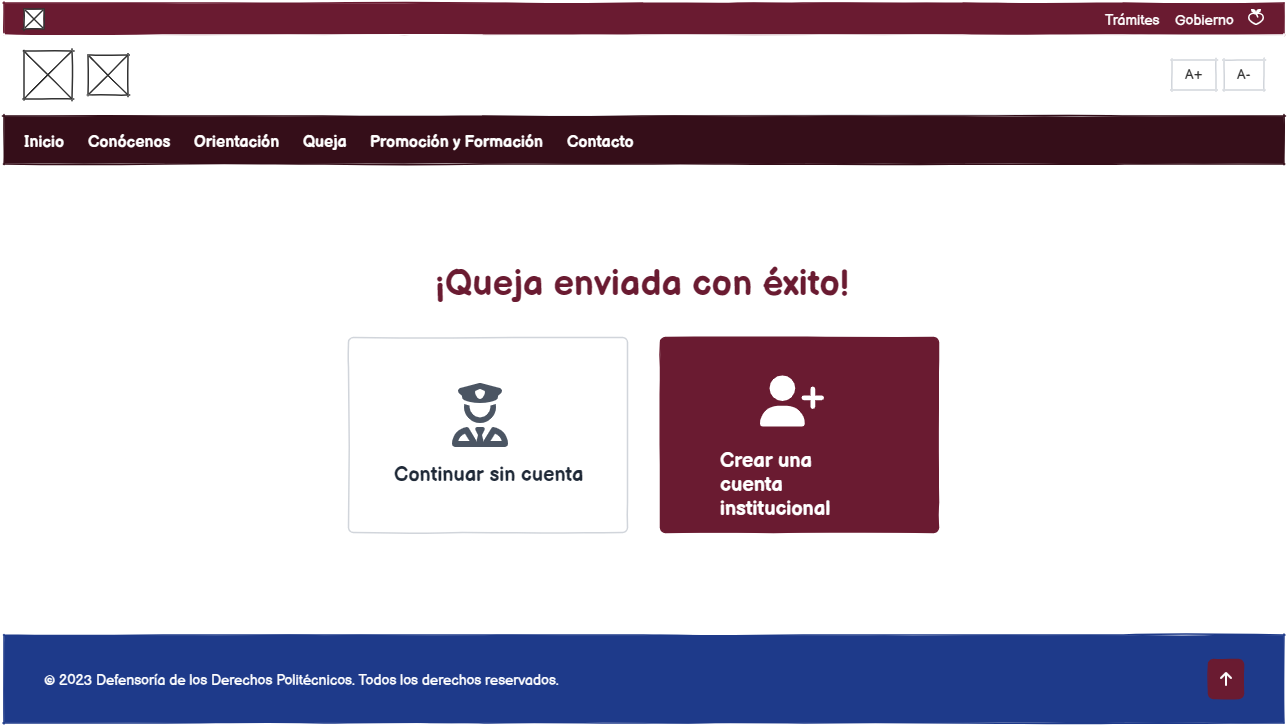
\includegraphics[width=0.85\textwidth]{imagenes/quejoso/QuejaEnviada.png}
    \caption{MQ-04: Pantalla de confirmación de envío exitoso.}
    \label{fig:mq04_exito}
\end{figure}

\noindent \textbf{Descripción de la interfaz (MQ-04):} \\
Una vez que el formulario es procesado correctamente, el sistema despliega esta pantalla de confirmación que asegura al usuario la recepción de su trámite. Los elementos de esta vista son:
\begin{itemize}
    \item \textbf{Mensaje de Éxito:} Un encabezado visualmente destacado que confirma el envío de la queja.
    \item \textbf{Opción "Continuar sin cuenta":} Permite al usuario finalizar el proceso de manera anónima o rápida, confiando en el folio que se le proporcione posteriormente para su seguimiento.
    \item \textbf{Opción "Crear una cuenta institucional":} Un botón de acción destacada que invita al usuario a registrarse formalmente. Esto facilita la gestión de múltiples trámites y el acceso a un historial personalizado dentro de la plataforma de la Defensoría.
\end{itemize}

\vspace{1cm}

% --- VISTA 05 ---
\begin{figure}[h]
    \centering
    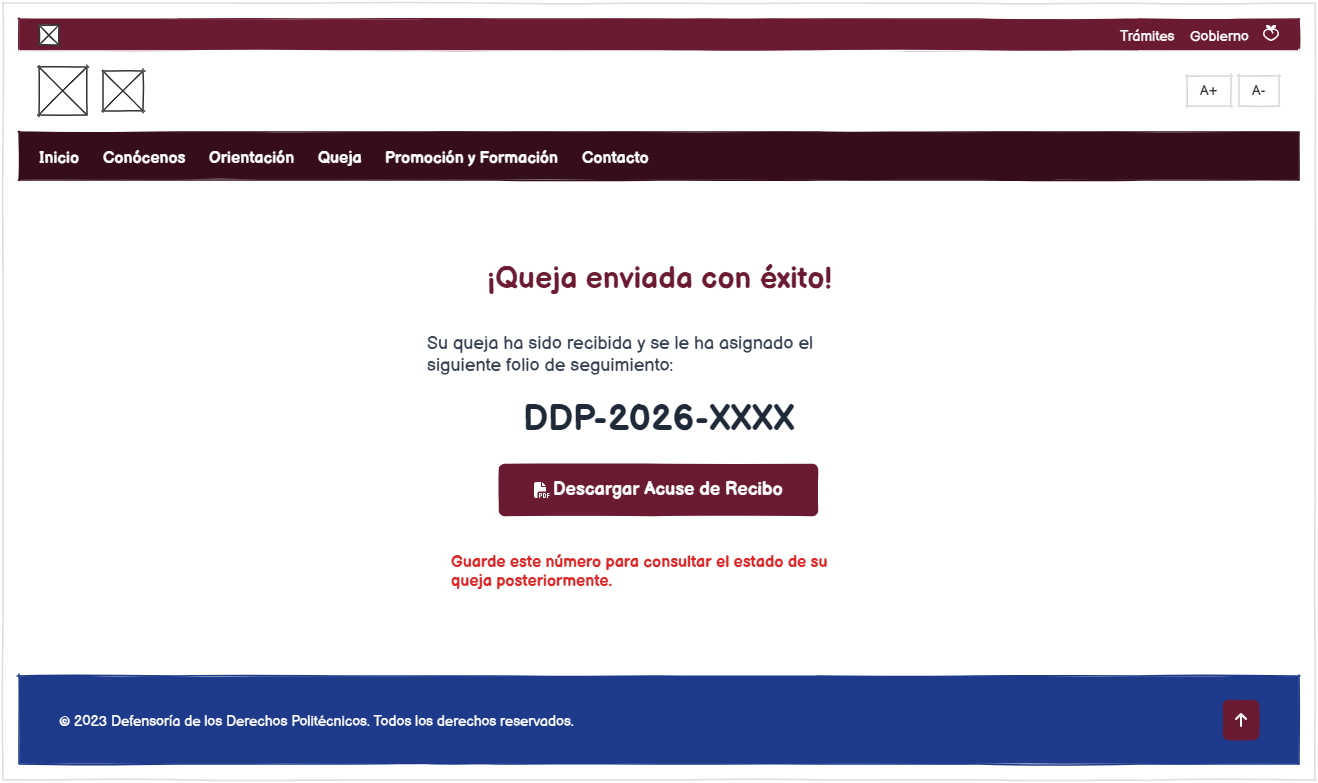
\includegraphics[width=0.85\textwidth]{imagenes/quejoso/FolioSeguimiento_NoCrearCuenta.png}
    \caption{MQ-05: Pantalla de finalización para usuarios sin registro de cuenta.}
    \label{fig:mq05_folio_sin_cuenta}
\end{figure}

\noindent \textbf{Descripción de la interfaz (MQ-05):} \\
Esta vista constituye el punto final del flujo para aquellos usuarios que optaron por la opción de "Continuar sin cuenta". :
\begin{itemize}
    \item \textbf{Asignación de Folio Único:} Se presenta el identificador alfanumérico generado por el sistema para permitir consultas externas futuras.
    \item \textbf{Generación de Comprobante:} Mantiene el botón de "Descargar Acuse de Recibo", siendo esta la única vía para que el usuario conserve los detalles de su queja fuera de la plataforma al no contar con un perfil personal.
    \item \textbf{Finalización del Flujo:} A diferencia de la versión con registro, se eliminan los botones de navegación hacia la configuración de cuenta, dejando el folio como el elemento central de la pantalla.
    \item \textbf{Instrucciones de Seguridad:} Se enfatiza mediante texto resaltado la responsabilidad del usuario de resguardar el folio, ya que es el único mecanismo de recuperación y seguimiento disponible para este perfil.
\end{itemize}

\vspace{1cm}

% --- VISTA 06 ---
\begin{figure}[h]
    \centering
    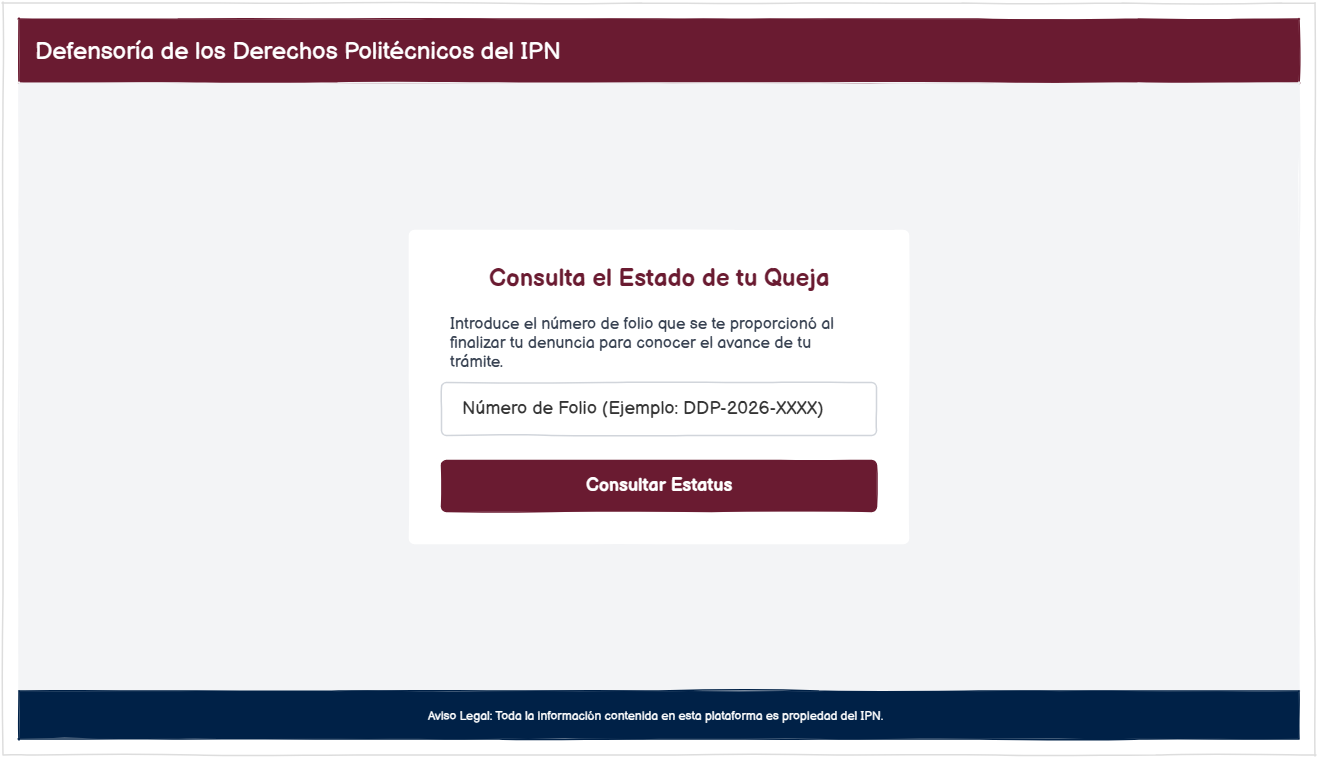
\includegraphics[width=0.85\textwidth]{imagenes/quejoso/ConsultaEstadoQueja.png}
    \caption{MQ-06: Interfaz de consulta de estado mediante folio.}
    \label{fig:mq06_consulta_folio}
\end{figure}

\noindent \textbf{Descripción de la interfaz (MQ-06):} \\
Esta interfaz permite a los usuarios que no cuentan con un perfil institucional o que desean una consulta rápida, verificar el avance de su solicitud. Los componentes principales son:
\begin{itemize}
    \item \textbf{Caja de Búsqueda Centrada:} Un contenedor visual que enfoca la atención del usuario en la tarea única de consulta, minimizando distracciones.
    \item \textbf{Campo de Entrada de Folio:} Espacio diseñado para introducir el código alfanumérico proporcionado al final del registro (ej. DDP-2026-XXXX). Incluye texto de ayuda (\textit{placeholder}) para orientar sobre el formato esperado.
    \item \textbf{Botón de Acción:} El control "Consultar Estatus" dispara la búsqueda en la base de datos de la Defensoría para recuperar la información vinculada a dicho folio.

\end{itemize}
\clearpage %

% --- VISTA 07 ---
\begin{figure}[h]
    \centering
    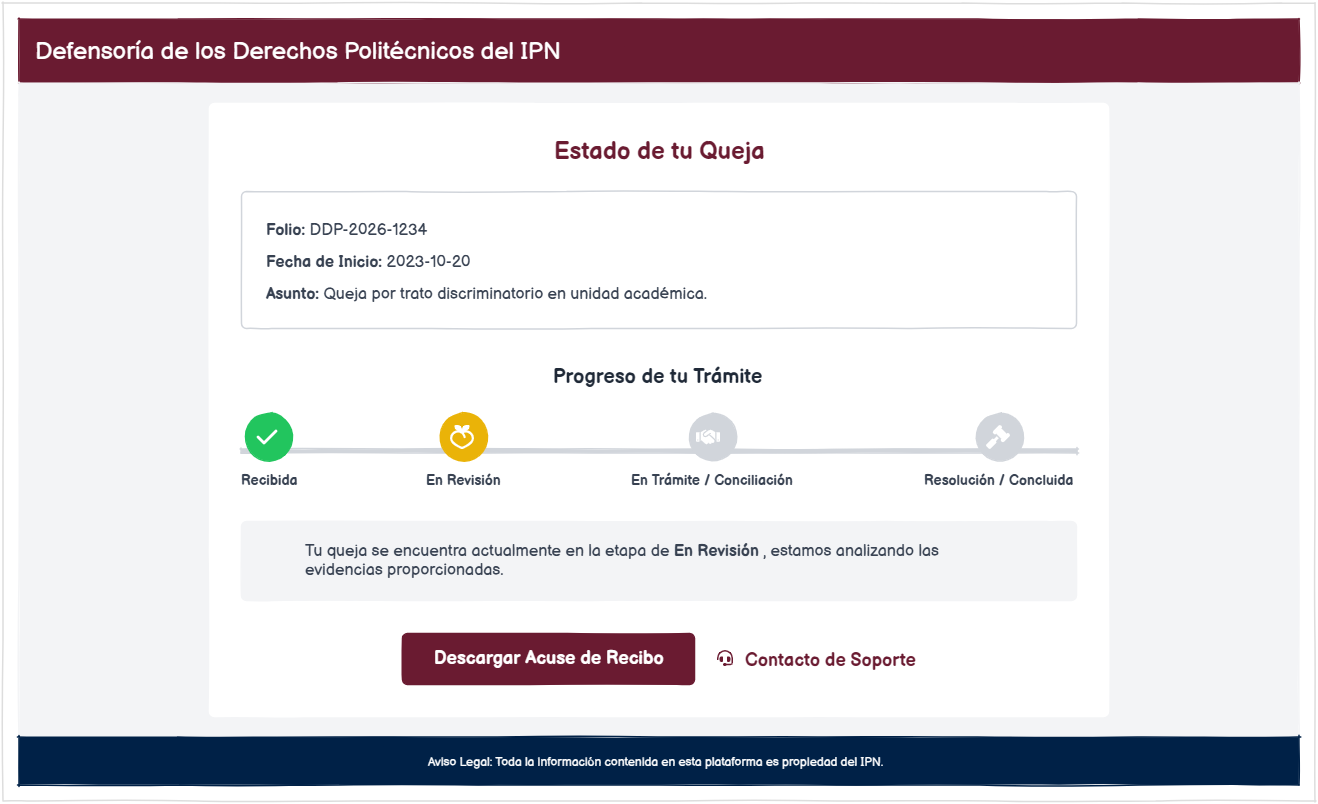
\includegraphics[width=0.85\textwidth]{imagenes/quejoso/EstadoQueja.png}
    \caption{MQ-07: Pantalla de visualización del estado y progreso del trámite.}
    \label{fig:mq07_estado_progreso}
\end{figure}

\noindent \textbf{Descripción de la interfaz (MQ-07):} \\
Esta pantalla proporciona una visión detallada y actualizada del estatus de una queja específica. Su diseño está orientado a reducir la incertidumbre del usuario mediante los siguientes componentes:
\begin{itemize}
    \item \textbf{Resumen del Expediente:} Recuadro informativo que muestra datos clave para confirmar la identidad del trámite: Folio (DDP-2026-1234), Fecha de Inicio y el Asunto breve.
    \item \textbf{Línea de Tiempo de Progreso:} Un indicador visual de pasos que muestra las etapas del proceso administrativo: Recibida, En Revisión, En Trámite / Conciliación y Resolución / Concluida. Los iconos cambian de color (verde y amarillo) para indicar etapas completadas o activas.
    \item \textbf{Mensaje de Estatus Detallado:} Un contenedor de texto que explica de manera clara y directa la situación actual ("estamos analizando las evidencias proporcionadas"), humanizando la interacción técnica.
    \item \textbf{Acciones de Usuario:} Incluye un botón para "Descargar Acuse de Recibo" (permitiendo recuperar el documento oficial en cualquier momento) y un acceso directo a Contacto de Soporte para dudas adicionales.
\end{itemize}

\vspace{1cm}
\vspace{1cm}
\vspace{1cm}
\vspace{1cm}



% --- VISTA 08 ---
\begin{figure}[h]
    \centering
    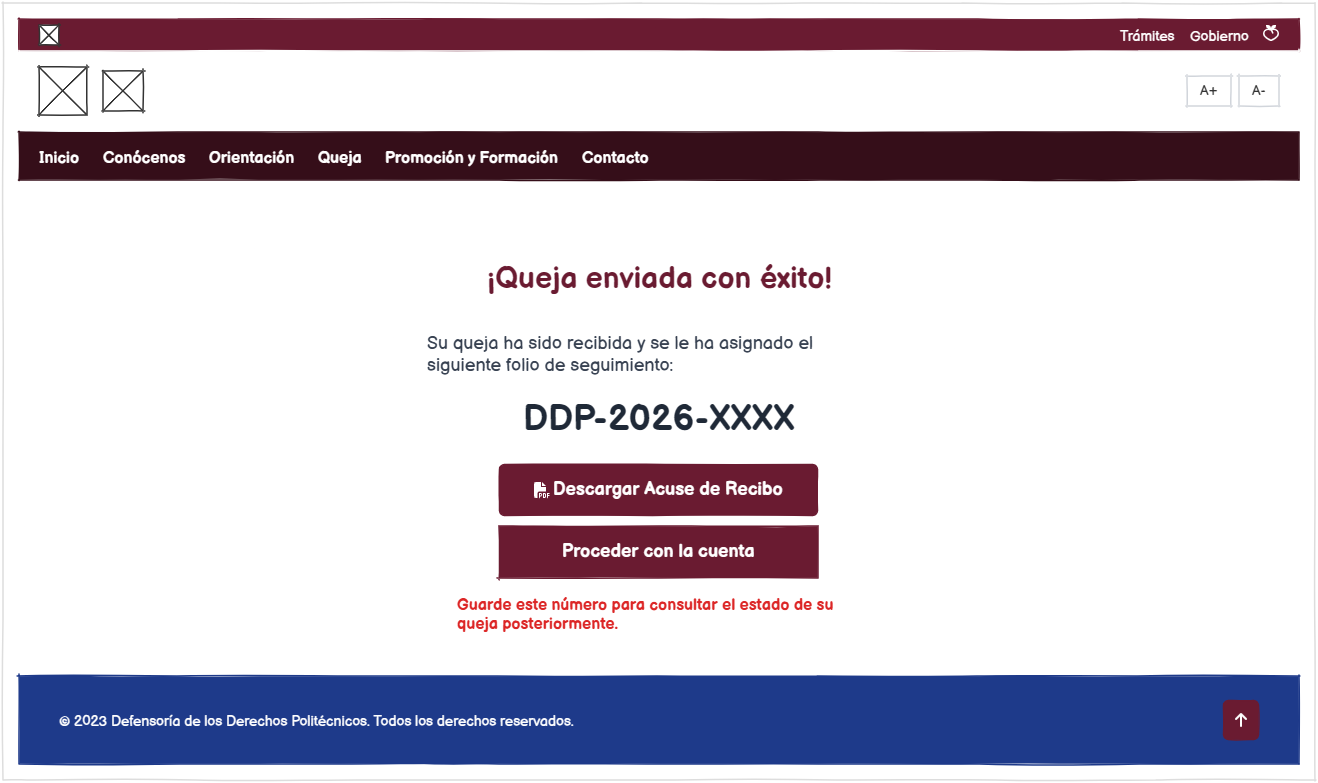
\includegraphics[width=0.85\textwidth]{imagenes/quejoso/FolioSeguimiento_CrearCuenta.png}
    \caption{MQ-08: Pantalla de asignación de folio y creación de cuenta.}
    \label{fig:mq05_folio}
\end{figure}

\noindent \textbf{Descripción de la interfaz (MQ-08):} \\
Esta pantalla es crucial para la transparencia del proceso, ya que proporciona al usuario la clave única para consultar el estado de su trámite. A diferencia de la vista MQ-05 la cual simplifica el tramite, esta busca crear una cuenta:
\begin{itemize}
    \item \textbf{Folio de Seguimiento:} Se muestra de forma prominente un código alfanumérico (ej. DDP-2026-XXXX) que servirá como referencia legal para el quejoso.
    \item \textbf{Descargar Acuse de Recibo:} Botón que permite generar un documento en formato PDF con el resumen de la queja enviada y el folio asignado, garantizando que el usuario tenga un respaldo físico o digital.
    \item \textbf{Proceder con la cuenta:} Botón de transición para aquellos usuarios que optaron por registrarse, dirigiéndolos al siguiente paso de creación de perfil.
    \item \textbf{Nota de Advertencia:} Texto de seguridad en color rojo que enfatiza la importancia de guardar el número de folio para consultas posteriores.
\end{itemize}

\clearpage %

% --- VISTA 09 ---
\begin{figure}[h]
    \centering
    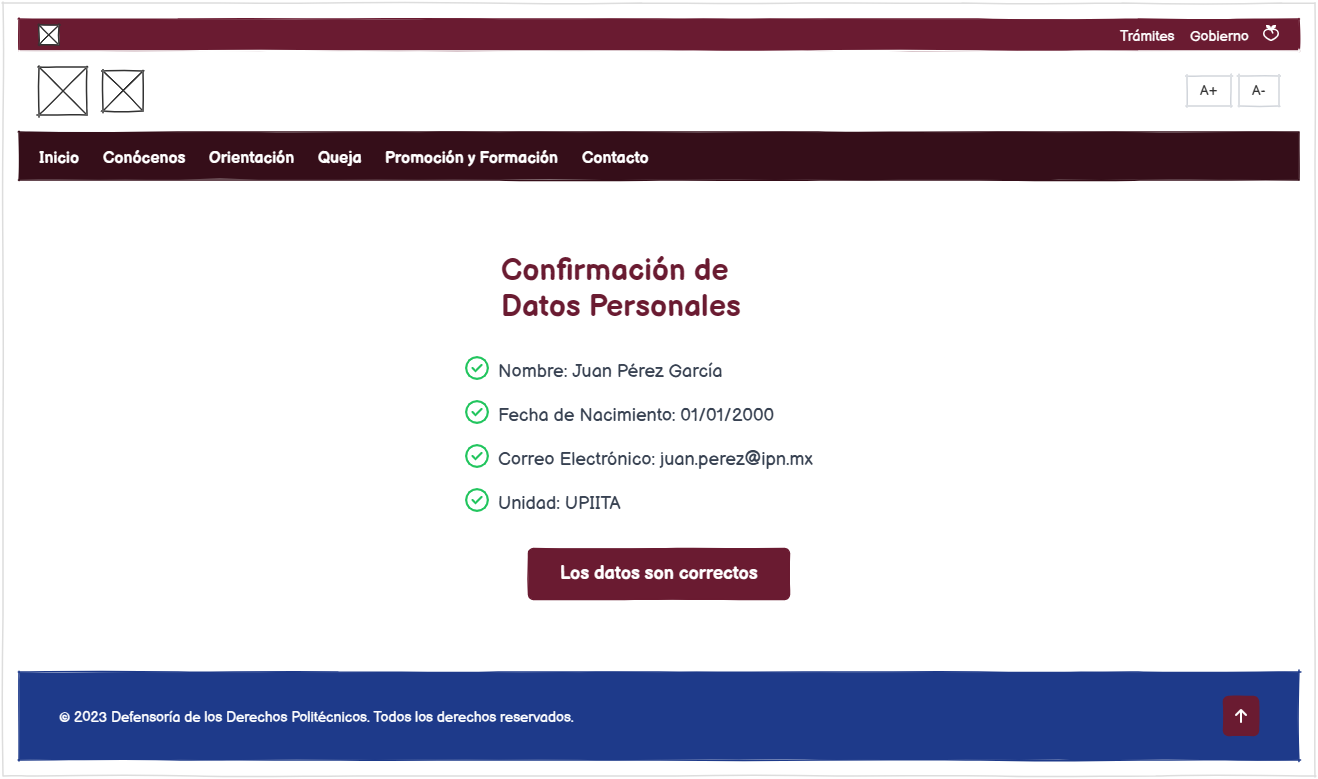
\includegraphics[width=0.85\textwidth]{imagenes/quejoso/ConfiguraciónDatosPersonales_CrearCuenta.png}
    \caption{MQ-09: Pantalla de confirmación de datos personales para registro.}
    \label{fig:mq06_confirmacion_datos}
\end{figure}

\noindent \textbf{Descripción de la interfaz (MQ-09):} \\
Tras optar por la creación de una cuenta institucional, el sistema presenta esta vista de verificación. Su objetivo es asegurar la integridad de la información vinculada al nuevo perfil. Los elementos clave son:
\begin{itemize}
    \item \textbf{Resumen de Identidad:} Listado de los datos capturados previamente (Nombre, Fecha de Nacimiento, Correo y Unidad), presentados con iconos de verificación para indicar que el formato es válido.
    \item \textbf{Vinculación Institucional:} Se muestra el correo con dominio institucional (ej. @ipn.mx) y la unidad académica (ej. UPIITA), reforzando la pertenencia a la comunidad politécnica.
    \item \textbf{Botón de Validación:} Control principal etiquetado como "Los datos son correctos", que actúa como disparador para la creación final del usuario en la base de datos.
    \item \textbf{Diseño Minimalista:} Se utiliza una disposición centralizada y limpia para enfocar la atención del usuario exclusivamente en la revisión de su información, minimizando errores de registro.
\end{itemize}

\clearpage %

% --- VISTA 10 ---
\begin{figure}[h]
    \centering
    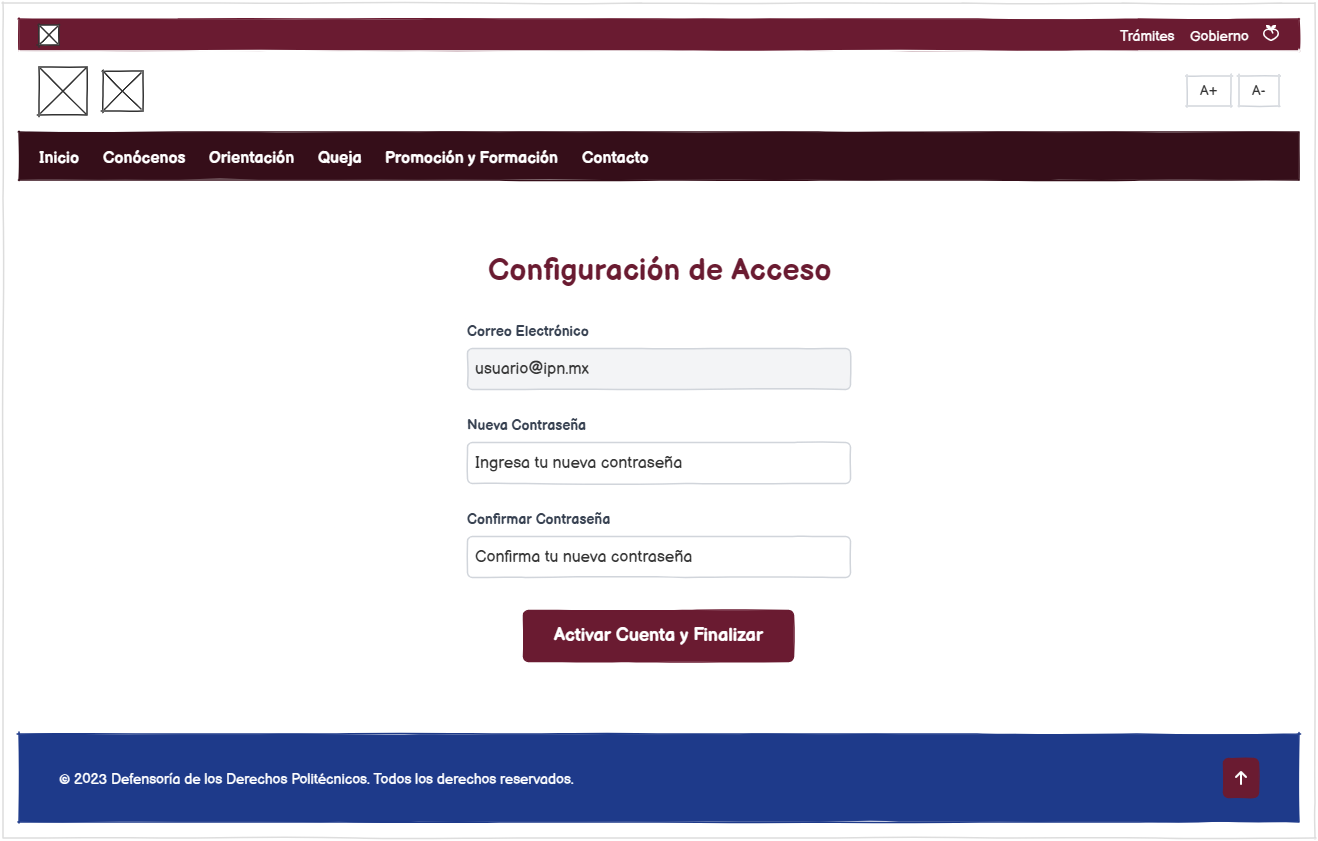
\includegraphics[width=0.85\textwidth]{imagenes/quejoso/ConfiguraciónAcceso_CrearCuenta.png}
    \caption{MQ-10: Pantalla de configuración de acceso y seguridad.}
    \label{fig:mq07_configuracion_acceso}
\end{figure}

\noindent \textbf{Descripción de la interfaz (MQ-10):} \\
Esta vista finaliza el proceso de registro mediante el establecimiento de las credenciales de seguridad del usuario. La interfaz se enfoca en la protección de la cuenta mediante los siguientes elementos:
\begin{itemize}
    \item \textbf{Identificador de Usuario:} Se muestra el correo electrónico institucional como el nombre de usuario invariable para el inicio de sesión.
    \item \textbf{Gestión de Contraseña:} Incluye dos campos de entrada de texto con máscara de seguridad para la creación y confirmación de la "Nueva Contraseña", asegurando que el usuario no cometa errores de escritura.
    \item \textbf{Finalización del Proceso:} El botón "Activar Cuenta y Finalizar" completa la transacción en el servidor, vinculando la queja inicial al nuevo perfil de usuario creado.
\end{itemize}

\clearpage %

% --- VISTA 11 ---
\begin{figure}[h]
    \centering
    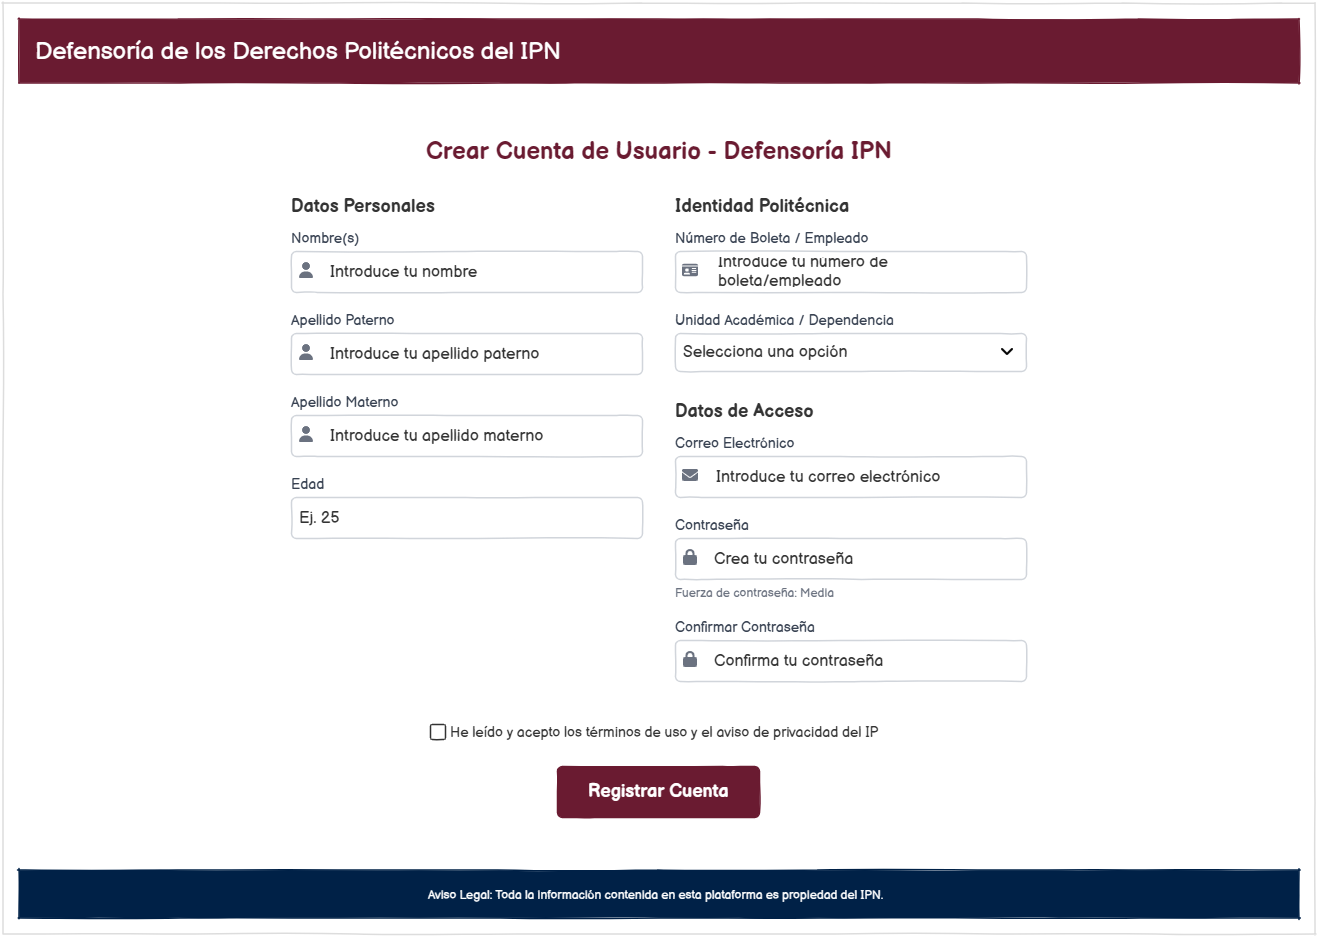
\includegraphics[width=0.85\textwidth]{imagenes/quejoso/CrearCuenta_Quejoso.png}
    \caption{MQ-11: Formulario general de creación de cuenta de usuario.}
    \label{fig:mq11_registro_general}
\end{figure}

\noindent \textbf{Descripción de la interfaz (MQ-11):} \\
Esta interfaz permite a cualquier miembro de la comunidad politécnica dar de alta un perfil en la plataforma de manera independiente. El formulario está organizado en tres secciones lógicas para facilitar la captura:
\begin{itemize}
    \item \textbf{Datos Personales:} Campos para el nombre(s), apellido paterno, apellido materno y edad. El uso de iconos dentro de los campos (\textit{input icons}) refuerza la claridad visual.
    \item \textbf{Identidad Politécnica:} Sección crítica para la validación institucional, solicitando el Número de Boleta o Empleado y la selección de la Unidad Académica o Dependencia mediante un menú desplegable.
    \item \textbf{Datos de Acceso:} Configuración del correo electrónico y establecimiento de contraseña. Incluye un indicador visual de "Fuerza de contraseña" para promover prácticas de seguridad robustas.
    \item \textbf{Validación Legal y Registro:} Incorpora un \textit{checkbox} obligatorio para la aceptación de los términos de uso y el aviso de privacidad del IPN, seguido del botón principal de "Registrar Cuenta".
\end{itemize}

\vspace{1cm}

% --- VISTA 12 ---
\begin{figure}[h]
    \centering
    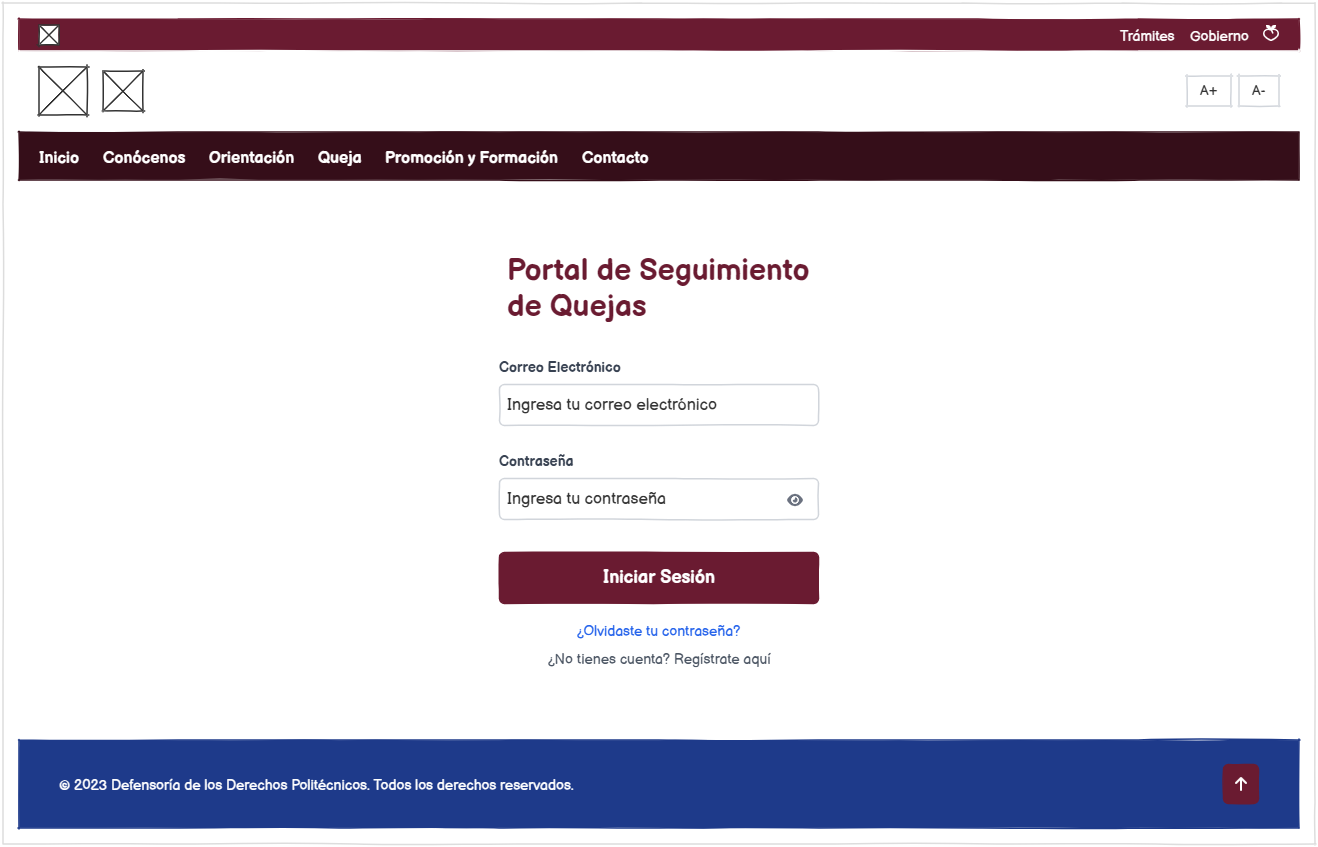
\includegraphics[width=0.85\textwidth]{imagenes/quejoso/InicioSesion_Quejoso.png}
    \caption{MQ-12: Interfaz de inicio de sesión para el portal de seguimiento.}
    \label{fig:mq12_login}
\end{figure}

\noindent \textbf{Descripción de la interfaz (MQ-12):} \\
Esta interfaz representa el punto de acceso para usuarios registrados (quejosos con cuenta institucional). Está diseñada para ser directa y segura, permitiendo la gestión personalizada de sus trámites. Los elementos clave son:
\begin{itemize}
    \item \textbf{Campos de Autenticación:} Entradas de texto para "Correo Electrónico" y "Contraseña". El campo de contraseña incluye un icono de visibilidad (ojo) para permitir al usuario verificar sus caracteres antes de enviar.
    \item \textbf{Botón de Acceso:} Un botón prominente de "Iniciar Sesión" que valida las credenciales contra el servidor de identidad.
    \item \textbf{Recuperación y Registro:} Incluye enlaces de soporte para usuarios que hayan olvidado su contraseña o para aquellos que aún no cuentan con un perfil y desean redirigirse al formulario de registro (MQ-11).
    \item \textbf{Encabezado Institucional:} Mantiene el menú de navegación completo, permitiendo al usuario volver a las secciones informativas o de orientación antes de autenticarse.
\end{itemize}

\vspace{1cm}

% --- VISTA 13 ---
\begin{figure}[h]
    \centering
    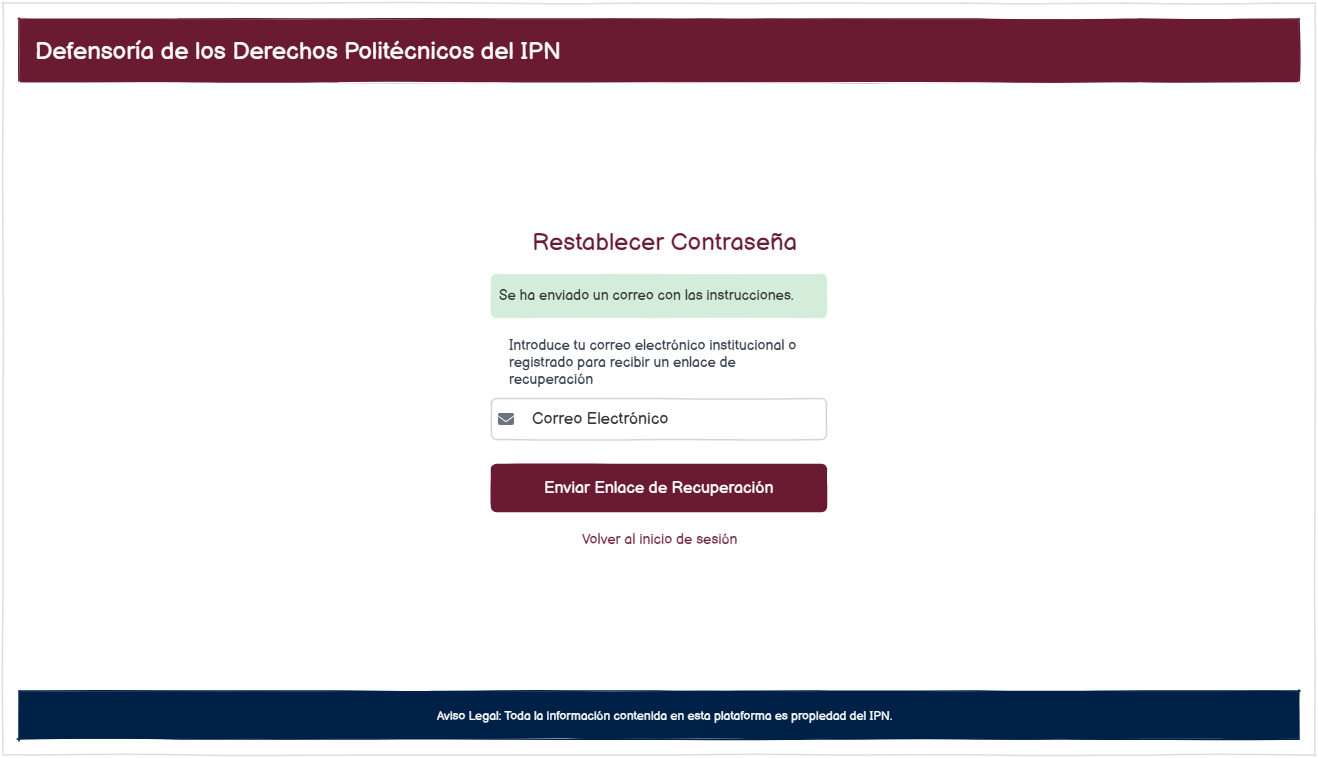
\includegraphics[width=0.85\textwidth]{imagenes/quejoso/RecuperarContraseña_Quejoso.png}
    \caption{MQ-13: Interfaz de restablecimiento de contraseña.}
    \label{fig:mq13_recuperar_pass}
\end{figure}

\noindent \textbf{Descripción de la interfaz (MQ-13):} \\
Esta vista proporciona un mecanismo de autoservicio para los usuarios que han perdido el acceso a su cuenta. La interfaz está diseñada para ser minimalista y funcional, centrada en una sola tarea de seguridad:
\begin{itemize}
    \item \textbf{Mensaje de Retroalimentación:} En la parte superior del formulario, se muestra una alerta visual (en color verde) que confirma al usuario cuando el sistema ha procesado satisfactoriamente el envío de las instrucciones por correo.
    \item \textbf{Instrucciones de Uso:} Un texto breve orienta al usuario para que introduzca su correo electrónico registrado, aclarando el propósito de la acción.
    \item \textbf{Campo de Correo Electrónico:} Entrada de datos única que cuenta con un icono de sobre para indicar semánticamente el tipo de información requerida.
    \item \textbf{Botón de Acción:} El control "Enviar Enlace de Recuperación" inicia el protocolo de seguridad para generar un token temporal de restablecimiento.
    \item \textbf{Enlace de Retorno:} Se incluye la opción "Volver al inicio de sesión" para facilitar la navegación en caso de que el usuario recuerde sus credenciales o haya accedido a esta vista por error.
\end{itemize}

\clearpage %

% --- VISTA 14 ---
\begin{figure}[h]
    \centering
    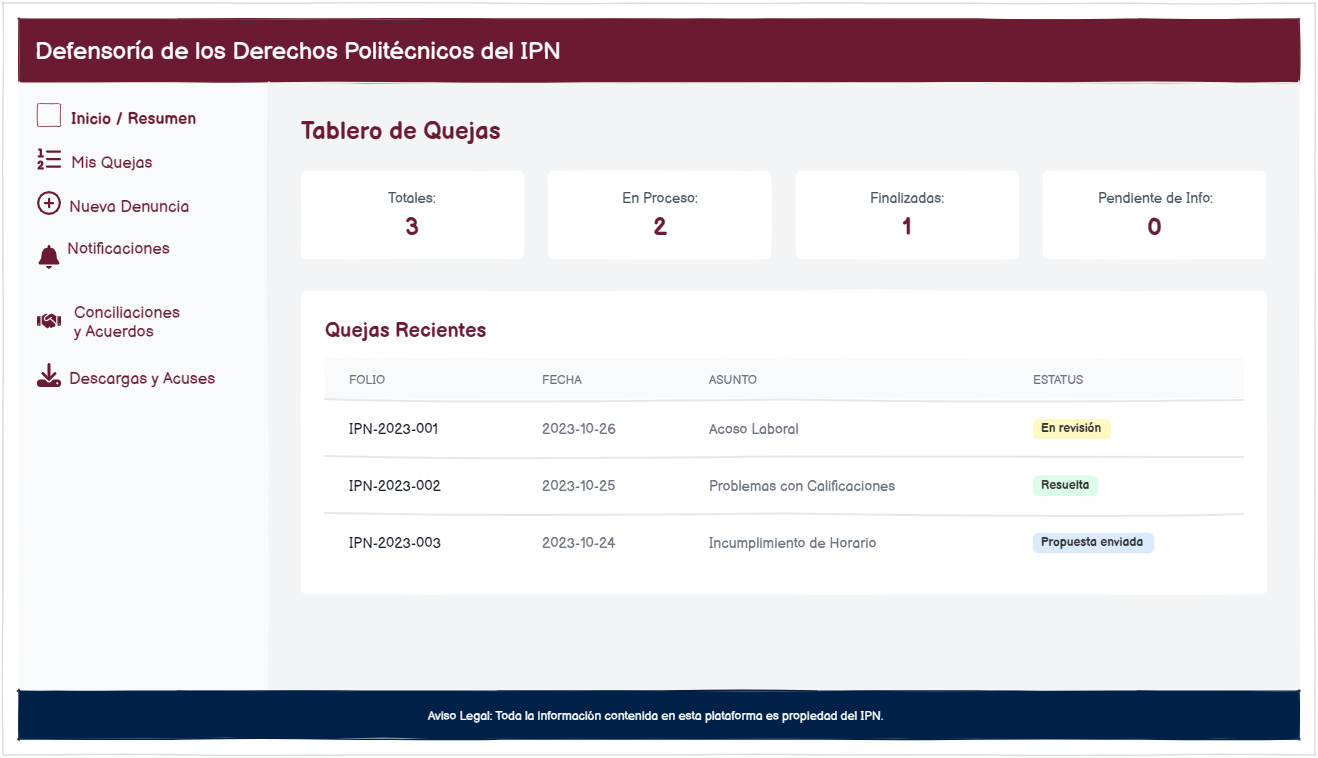
\includegraphics[width=0.85\textwidth]{imagenes/quejoso/Dashboard_Quejoso.png}
    \caption{MQ-14: Tablero de control principal del usuario registrado.}
    \label{fig:mq14_dashboard}
\end{figure}

\noindent \textbf{Descripción de la interfaz (MQ-14):} \\
Esta pantalla constituye el centro de mando del quejoso una vez iniciada la sesión. Está diseñada para ofrecer información estadística y operativa de manera inmediata. Los componentes principales son:
\begin{itemize}
    \item \textbf{Menú Lateral de Navegación:} Un panel a la izquierda que organiza las funciones clave: Resumen, Listado de Quejas, Nueva Denuncia, Notificaciones, Conciliaciones y un repositorio de Descargas. Cada opción cuenta con iconografía representativa.
    \item \textbf{Tarjetas de Resumen Estadístico:} Cuatro indicadores cuantitativos que muestran el estado general de las solicitudes: Totales, En Proceso, Finalizadas y Pendientes de Información. Esto permite una monitorización rápida del avance global.
    \item \textbf{Tabla de Quejas Recientes:} Un listado detallado que muestra las últimas interacciones del usuario, incluyendo el folio institucional, la fecha de registro, el asunto de la denuncia y el estatus actual diferenciado por etiquetas de color (ej. En revisión, Resuelta, Propuesta enviada).
    \item \textbf{Barra de Identidad:} Mantenimiento de la identidad gráfica institucional en el encabezado y pie de página, garantizando un entorno formal y confiable para la gestión de derechos.
\end{itemize}

\clearpage %

% --- VISTA 15 ---
\begin{figure}[h]
    \centering
    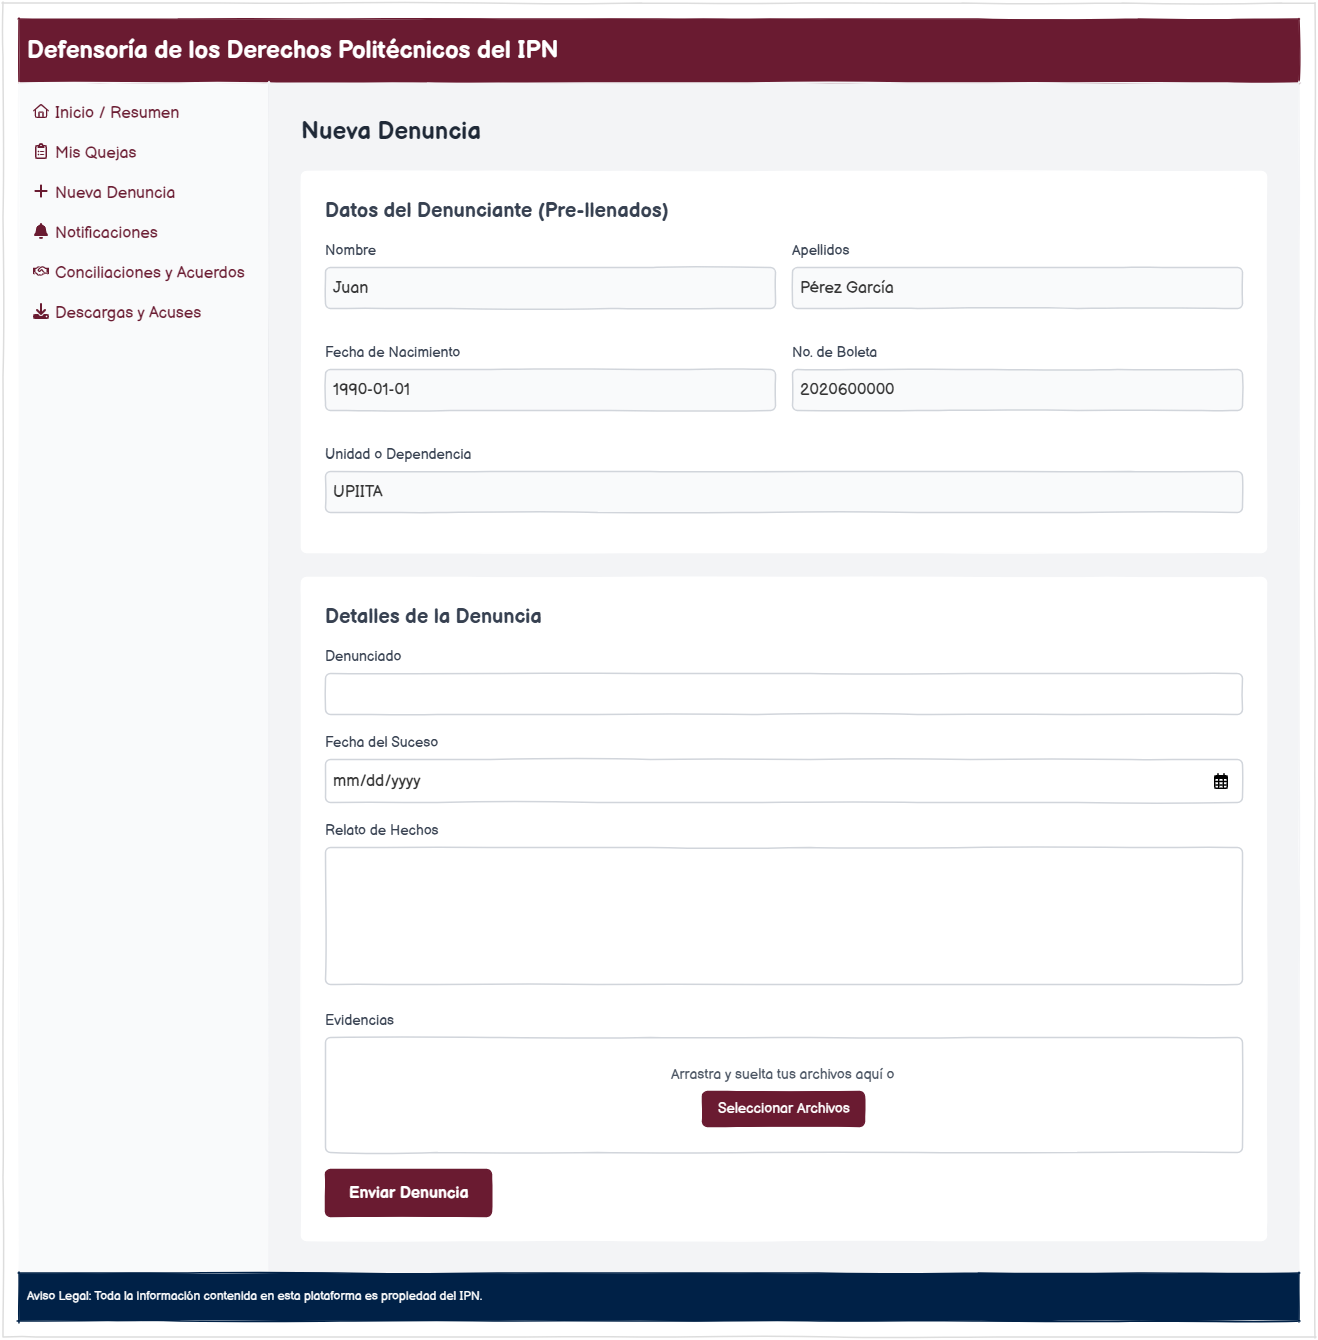
\includegraphics[width=0.85\textwidth]{imagenes/quejoso/NuevaQueja.png}
    \caption{MQ-15: Formulario de nueva denuncia para usuario autenticado.}
    \label{fig:mq15_nueva_queja_auth}
\end{figure}

\noindent \textbf{Descripción de la interfaz (MQ-15):} \\
Esta interfaz representa la optimización del proceso de denuncia para usuarios con cuenta activa. A diferencia del formulario general, esta vista integra la información del perfil para agilizar el trámite. Sus componentes son:
\begin{itemize}
    \item \textbf{Datos del Denunciante (Pre-llenados):} El sistema recupera automáticamente el nombre, apellidos, fecha de nacimiento, número de boleta y unidad académica de la base de datos. Estos campos aparecen en modo de solo lectura o validados, eliminando la carga de datos repetitiva.
    \item \textbf{Detalles de la Denuncia:} Sección activa para la captura de la información específica del incidente, incluyendo el nombre del denunciado, la fecha del suceso y el relato de los hechos.
    \item \textbf{Gestión de Evidencias:} Área de carga de archivos que implementa la función de arrastrar y soltar (\textit{drag and drop}) o selección manual, facilitando la adjunción de pruebas documentales o multimedia.
    \item \textbf{Navegación Contextual:} Se mantiene el menú lateral del \textit{dashboard}, permitiendo al usuario interrumpir el proceso o consultar otras secciones sin perder la consistencia visual del panel de control.
\end{itemize}

\vspace{1cm}

% --- VISTA 16 ---
\begin{figure}[h]
    \centering
    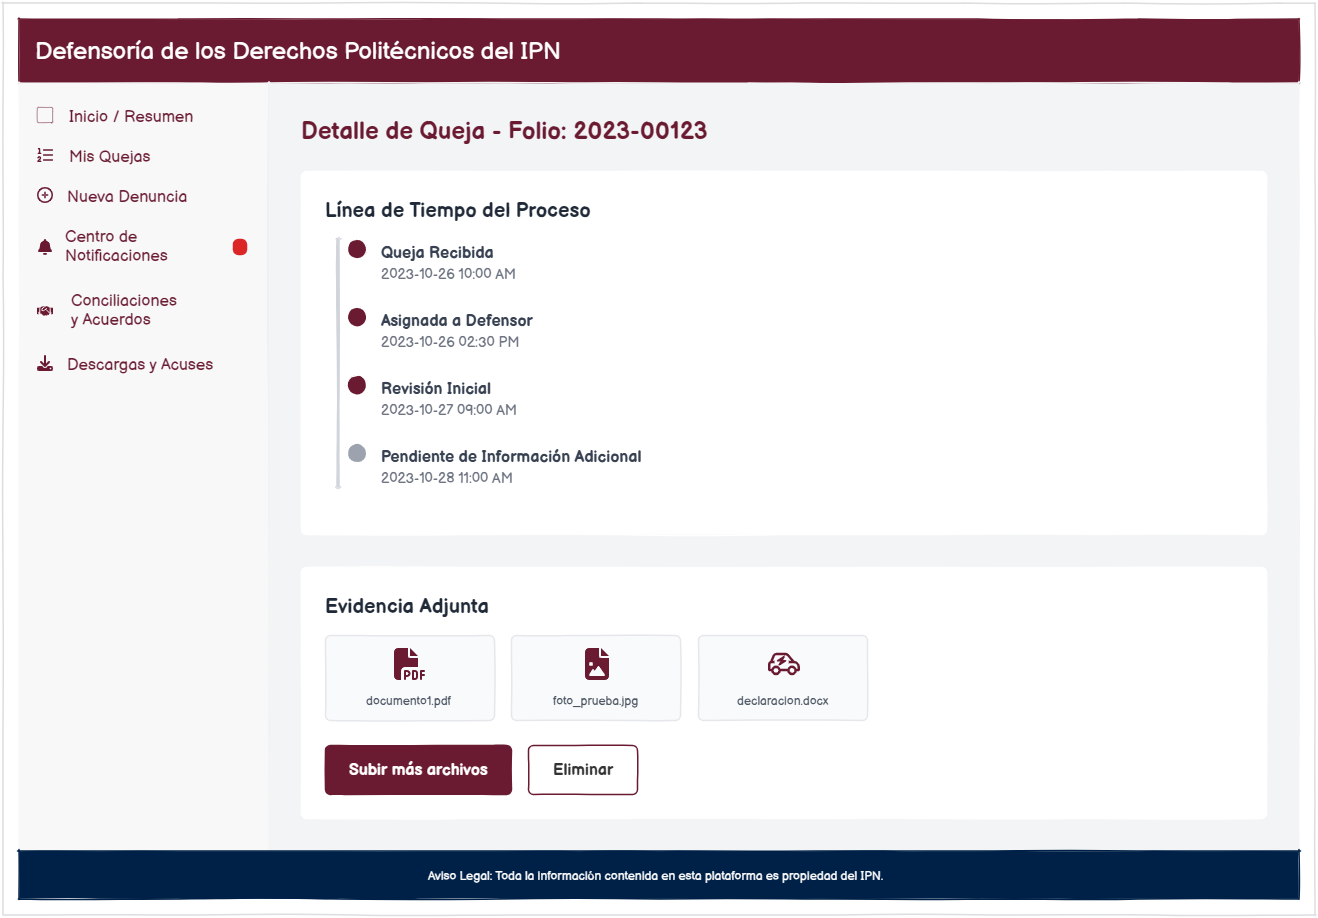
\includegraphics[width=0.85\textwidth]{imagenes/quejoso/DetallesyEvidenciaQujea.png}
    \caption{MQ-16: Detalle de expediente con línea de tiempo y gestión de evidencias.}
    \label{fig:mq16_detalle_evidencias}
\end{figure}

\noindent \textbf{Descripción de la interfaz (MQ-16):} \\
Esta pantalla permite al usuario profundizar en el estado de una queja en particular, ofreciendo herramientas para la interacción activa con su expediente. Los elementos destacados son:
\begin{itemize}
    \item \textbf{Línea de Tiempo del Proceso:} Un registro histórico vertical que detalla cada hito del trámite con fecha y hora exacta. Incluye estados como "Queja Recibida", "Asignada a Defensor", "Revisión Inicial" y estados pendientes, proporcionando una auditoría clara del flujo de trabajo.
    \item \textbf{Gestión de Evidencia Adjunta:} Un panel que muestra los archivos cargados previamente (documentos PDF, imágenes JPG, archivos Word). Cada archivo se presenta con un icono representativo de su formato para una rápida identificación.
    \item \textbf{Controles de Archivos:} Botones de acción que permiten al usuario "Subir más archivos" (en caso de que la Defensoría solicite información adicional) otorgando control sobre la documentación presentada.
    \item \textbf{Indicador de Notificaciones:} En el menú lateral se observa un distintivo visual (punto rojo) en el "Centro de Notificaciones", alertando al usuario sobre nuevas actualizaciones o requerimientos pendientes en su expediente.
\end{itemize}

\vspace{0.5cm}

% --- VISTA 17 ---
\begin{figure}[h]
    \centering
    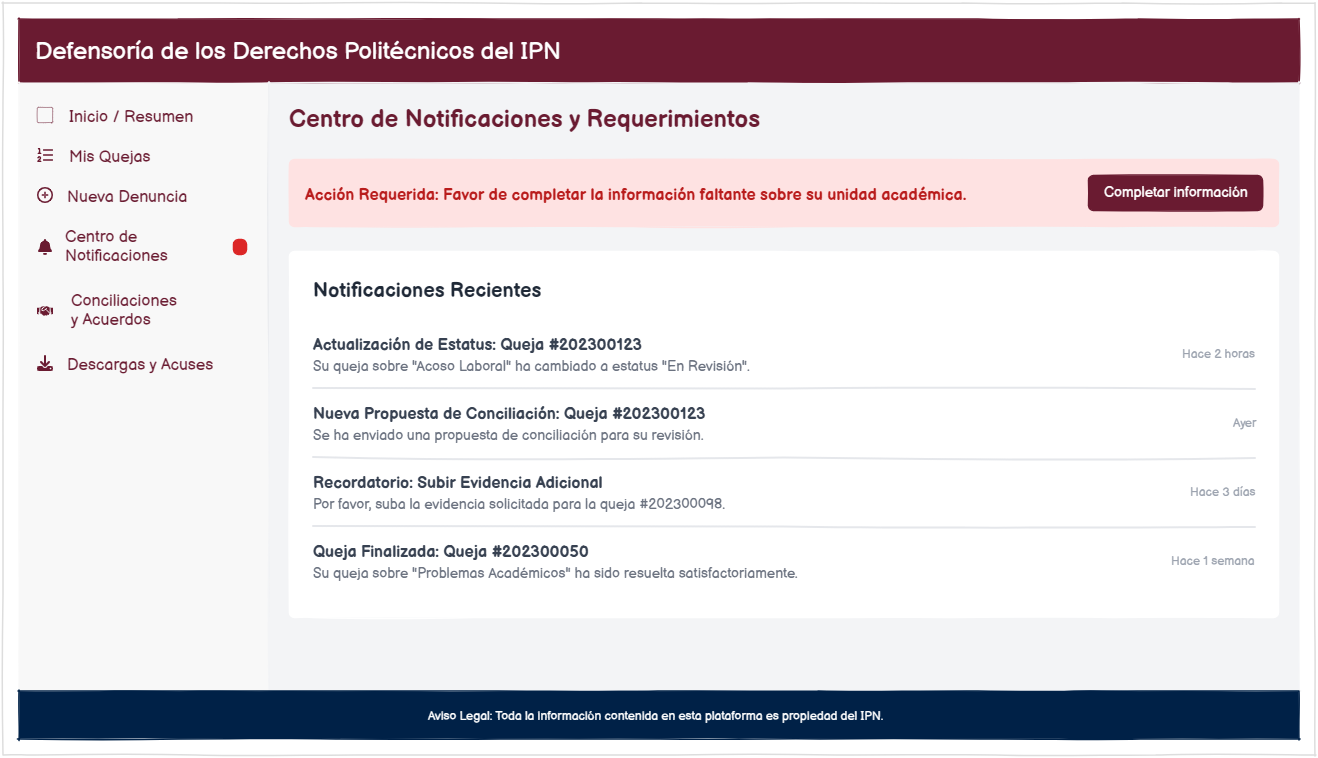
\includegraphics[width=0.85\textwidth]{imagenes/quejoso/NotificacionesRequerimientos.png}
    \caption{MQ-17: Centro de notificaciones y gestión de requerimientos.}
    \label{fig:mq17_notificaciones}
\end{figure}

\noindent \textbf{Descripción de la interfaz (MQ-17):} \\
Esta pantalla centraliza las alertas y solicitudes de información dirigidas al usuario, permitiendo una comunicación fluida y trazable. Los componentes clave son:
\begin{itemize}
    \item \textbf{Banner de Acción Requerida:} Un contenedor de alta prioridad en color rojo que destaca solicitudes críticas (ej. falta de información sobre la unidad académica). Incluye un botón de acceso directo ("Completar información") para resolver el requerimiento de inmediato.
    \item \textbf{Historial de Notificaciones:} Un listado cronológico de eventos relevantes relacionados con los expedientes del usuario. Cada elemento muestra un título claro, una breve descripción del suceso y el tiempo transcurrido (ej. "Hace 2 horas", "Ayer").
    \item \textbf{Tipología de Alertas:} El sistema categoriza los mensajes en actualizaciones de estatus, propuestas de conciliación, recordatorios de evidencia y avisos de finalización, permitiendo al usuario identificar la naturaleza de cada aviso a simple vista.
    \item \textbf{Navegación Persistente:} El indicador visual en el menú lateral permanece activo mientras existan notificaciones no leídas, asegurando que el quejoso esté al tanto de cualquier necesidad administrativa para el avance de su trámite.
\end{itemize}
% ------------------------------------------------------------------------------
% SECCIÓN 2: PERFIL ADMINISTRACIÓN Y DEFENSORÍA
% ------------------------------------------------------------------------------
\section{Perfil: Administración y Defensoría}
Este perfil integra las herramientas de gestión interna de la plataforma. El acceso está restringido al personal de la Defensoría de los Derechos Politécnicos y se divide en cuatro departamentos operativos con facultades diferenciadas para garantizar la debida atención de los expedientes.

% --- VISTA ADMINISTRATIVA 01 ---
\begin{figure}[h]
    \centering
    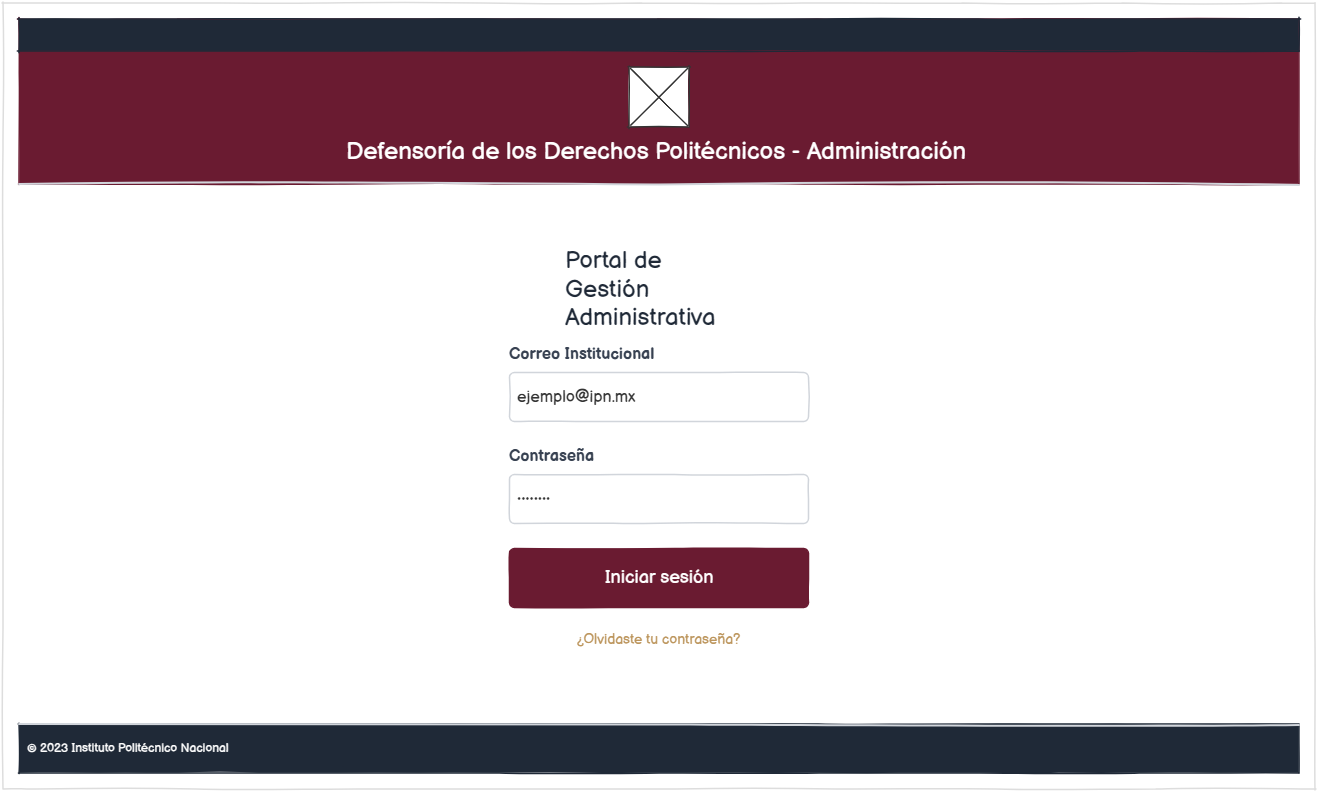
\includegraphics[width=0.85\textwidth]{imagenes/recepcion/InicioSesión_DDP.png}
    \caption{MA-01: Portal de acceso al Sistema de Gestión Administrativa.}
    \label{fig:ma01_login_adm}
\end{figure}

\noindent \textbf{Descripción de la interfaz (MA-01):} \\
Esta interfaz representa el punto de acceso unificado para el personal de la Defensoría de los Derechos Politécnicos. A diferencia del portal ciudadano, esta vista está optimizada para la seguridad interna. Sus elementos incluyen:
\begin{itemize}
    \item \textbf{Encabezado de Administración:} Identificación clara del módulo administrativo para evitar confusiones con el portal de quejosos.
    \item \textbf{Campos de Credenciales:} Entradas para correo institucional y contraseña, vinculadas al directorio activo de la institución para garantizar que solo personal autorizado acceda.
    \item \textbf{Gestión de Sesión:} Botón de "Iniciar sesión" y enlace de recuperación de contraseña.
    \item \textbf{Identidad Institucional:} Pie de página oficial del Instituto Politécnico Nacional, reforzando el carácter normativo del portal.
\end{itemize}

\vspace{1cm}

% --- VISTA ADMINISTRATIVA 02 ---
\begin{figure}[h]
    \centering
    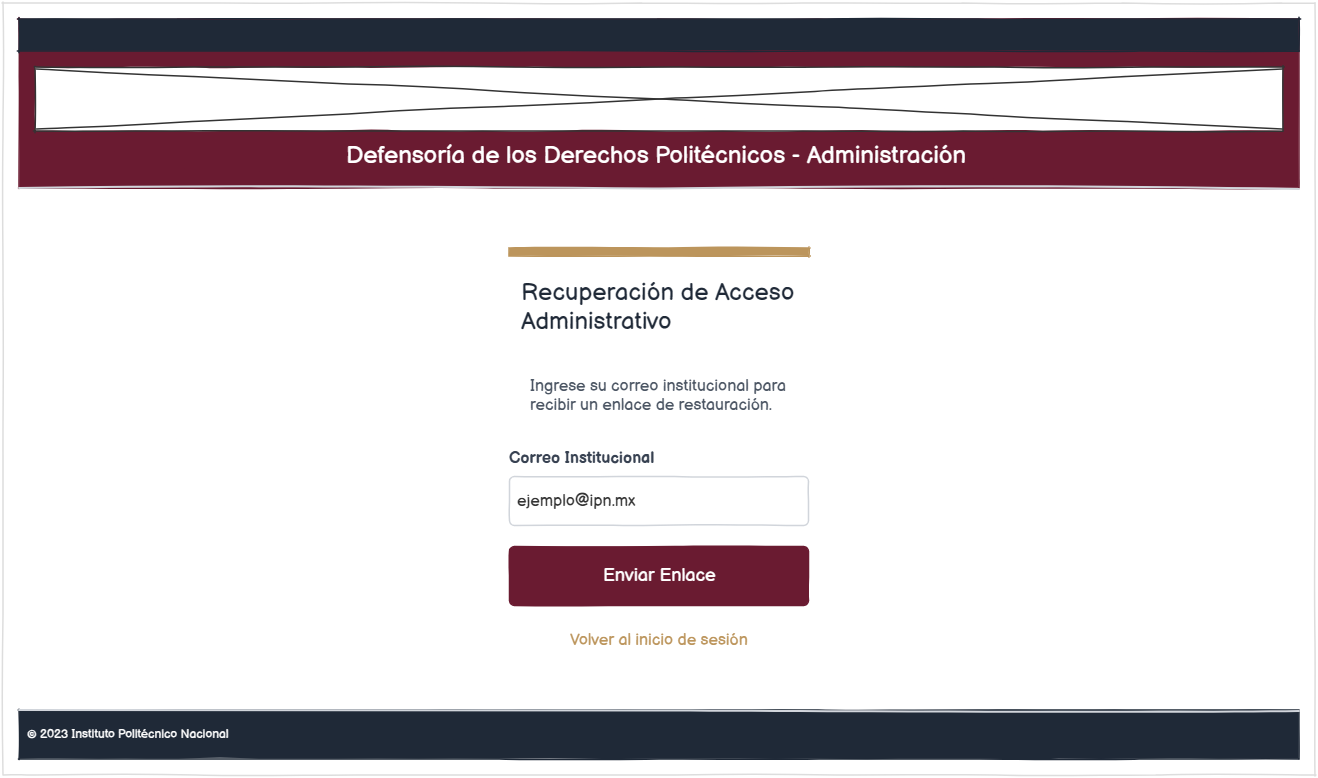
\includegraphics[width=0.85\textwidth]{imagenes/recepcion/RecuperaciónContraseñaDDP.png}
    \caption{MA-02: Interfaz de recuperación de acceso para personal administrativo.}
    \label{fig:ma02_recuperar_adm}
\end{figure}

\noindent \textbf{Descripción de la interfaz (MA-02):} \\
Esta vista permite al personal de los cuatro departamentos (Recepción, Primer Contacto, Subdefensoría y Defensoría) restablecer sus credenciales de acceso de manera autónoma. Los componentes destacados son:
\begin{itemize}
    \item \textbf{Validación Institucional:} El sistema requiere exclusivamente el correo institucional para procesar la solicitud, asegurando que el enlace de restauración se envíe a una cuenta oficial.
    \item \textbf{Flujo de Recuperación:} Un diseño simplificado que guía al usuario mediante instrucciones directas para recibir el enlace de restauración.
    \item \textbf{Control de Navegación:} Enlace para Volver al inicio de sesión en caso de que el usuario requiera cancelar la acción o haya recordado sus datos.
\end{itemize}

\vspace{1cm}

\subsection{Departamento de Recepción}
Es el primer filtro del sistema, encargado de la validación inicial de los datos de entrada y la asignación preliminar de folios o turnos.

\begin{figure}[h]
    \centering
    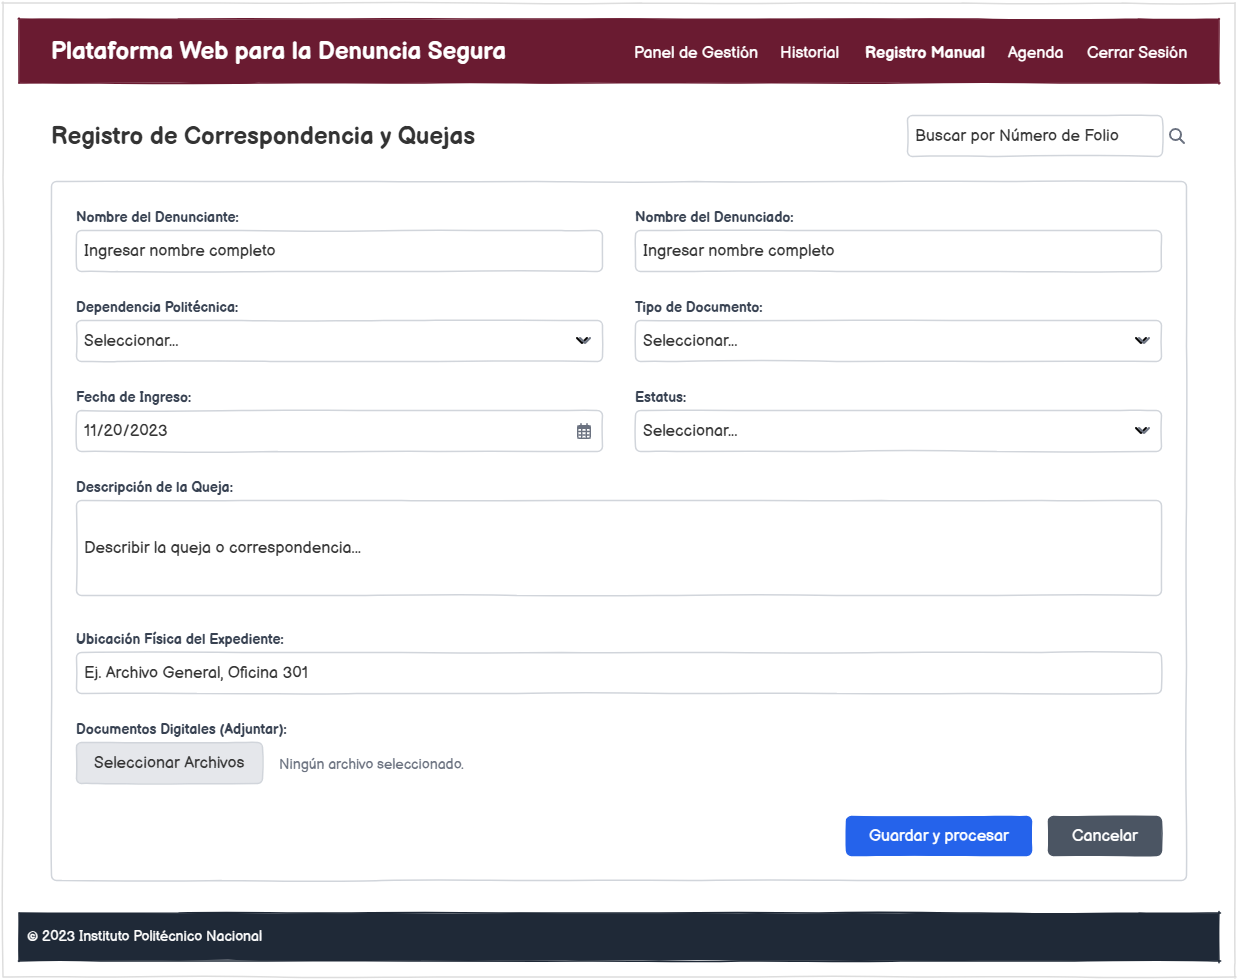
\includegraphics[width=0.85\textwidth]{imagenes/recepcion/RegistroManualQueja.png}
    \caption{MA-03: Formulario de registro manual de correspondencia y quejas.}
    \label{fig:ma03_registro_manual}
\end{figure}

\noindent \textbf{Descripción de la interfaz (MA-03):} \\
Esta interfaz permite al personal administrativo registrar quejas o correspondencia recibida de manera presencial o mediante oficialía de partes. El diseño facilita la creación de un "gemelo digital" del expediente físico mediante los siguientes componentes:
\begin{itemize}
    \item \textbf{Buscador de Folio:} Ubicado en la parte superior derecha, permite verificar rápidamente si un expediente ya existe en la base de datos antes de duplicar el registro.
    \item \textbf{Datos del Sujeto:} Campos específicos para capturar el nombre completo tanto del denunciante como del denunciado.
    \item \textbf{Clasificación Administrativa:} Selectores desplegables para definir la Dependencia Politécnica, el Tipo de Documento y el Estatus inicial del trámite.
    \item \textbf{Ubicación de Archivo Físico:} Campo especializado para registrar el lugar exacto de resguardo del papel original (ej. Archivo General, estantería u oficina), garantizando la trazabilidad entre lo digital y lo físico.
    \item \textbf{Carga de Evidencia Digital:} Botón para adjuntar escaneos o fotos de los documentos recibidos, integrándolos inmediatamente al repositorio del sistema.
\end{itemize}
\vspace{1cm}

% --- VISTA 04: PANEL DE GESTIÓN ---
\begin{figure}[h]
    \centering
    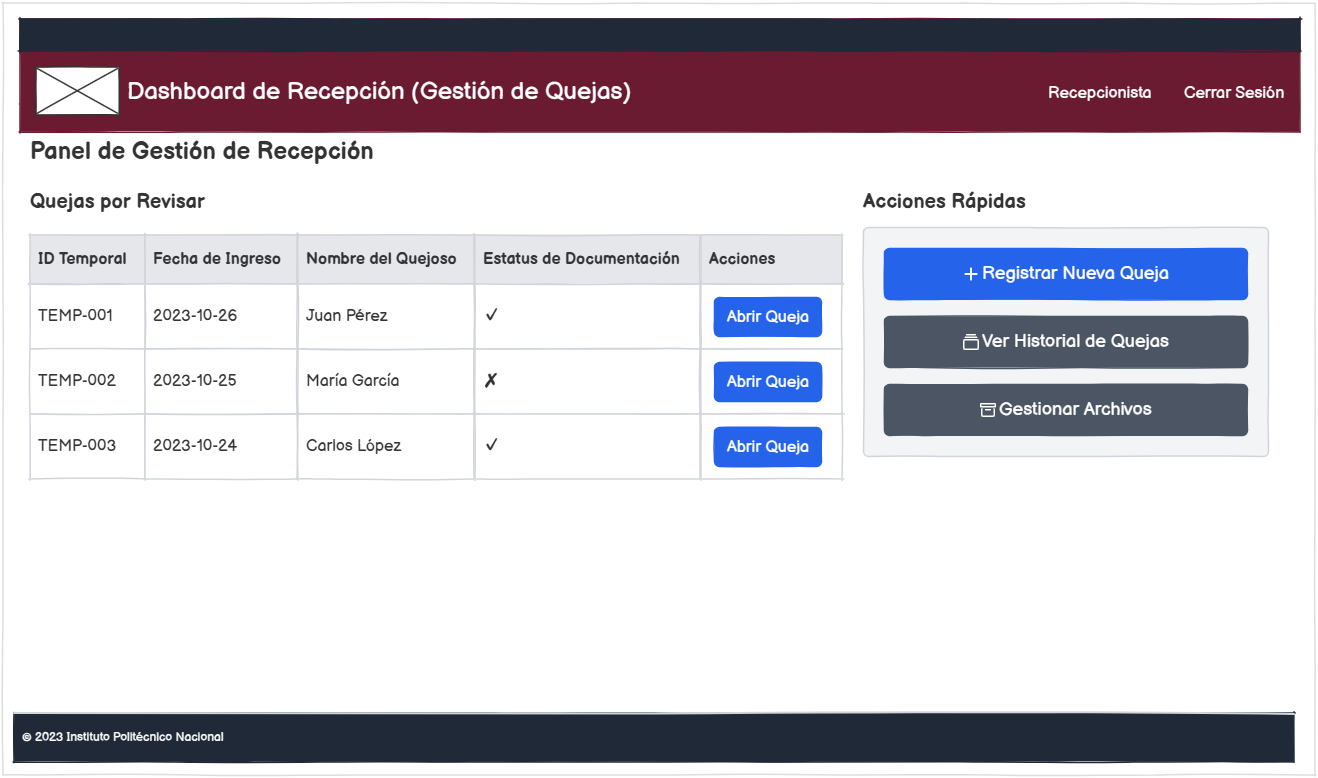
\includegraphics[width=0.85\textwidth]{imagenes/recepcion/PanelGestiónRecepción.png}
    \caption{MA-04: Panel de gestión de recepción (Dashboard).}
    \label{fig:ma04_dashboard_recepcion}
\end{figure}

\noindent \textbf{Descripción de la interfaz (MA-04):} \\
Este tablero de control permite al personal de recepción monitorear y administrar las quejas entrantes de manera centralizada. Sus componentes principales son:
\begin{itemize}
    \item \textbf{Listado de Quejas por Revisar:} Una tabla operativa que muestra los registros pendientes. Utiliza un sistema de "ID Temporal" para identificar las quejas que aún no han sido validadas o canalizadas.
    \item \textbf{Indicador de Documentación:} Columna visual que utiliza iconos (check o cruz) para señalar de forma rápida si un expediente cuenta con la documentación digital completa o si requiere atención inmediata.
    \item \textbf{Acceso Directo al Expediente:} El botón "Abrir Queja" permite al recepcionista entrar al detalle de cada registro para proceder con su validación técnica.
    \item \textbf{Menú de Acciones Rápidas:} Panel lateral derecho que facilita las tareas más frecuentes: registrar una nueva queja, consultar el historial histórico de registros o acceder al repositorio general de archivos.
    \item \textbf{Identificación de Rol:} El encabezado muestra el perfil activo ("Recepcionista"), asegurando que el usuario sea consciente de sus permisos dentro del sistema de administración.
\end{itemize}

\vspace{1cm}

% --- VISTA 05: VALIDACIÓN DE REQUISITOS ---
\begin{figure}[h]
    \centering
    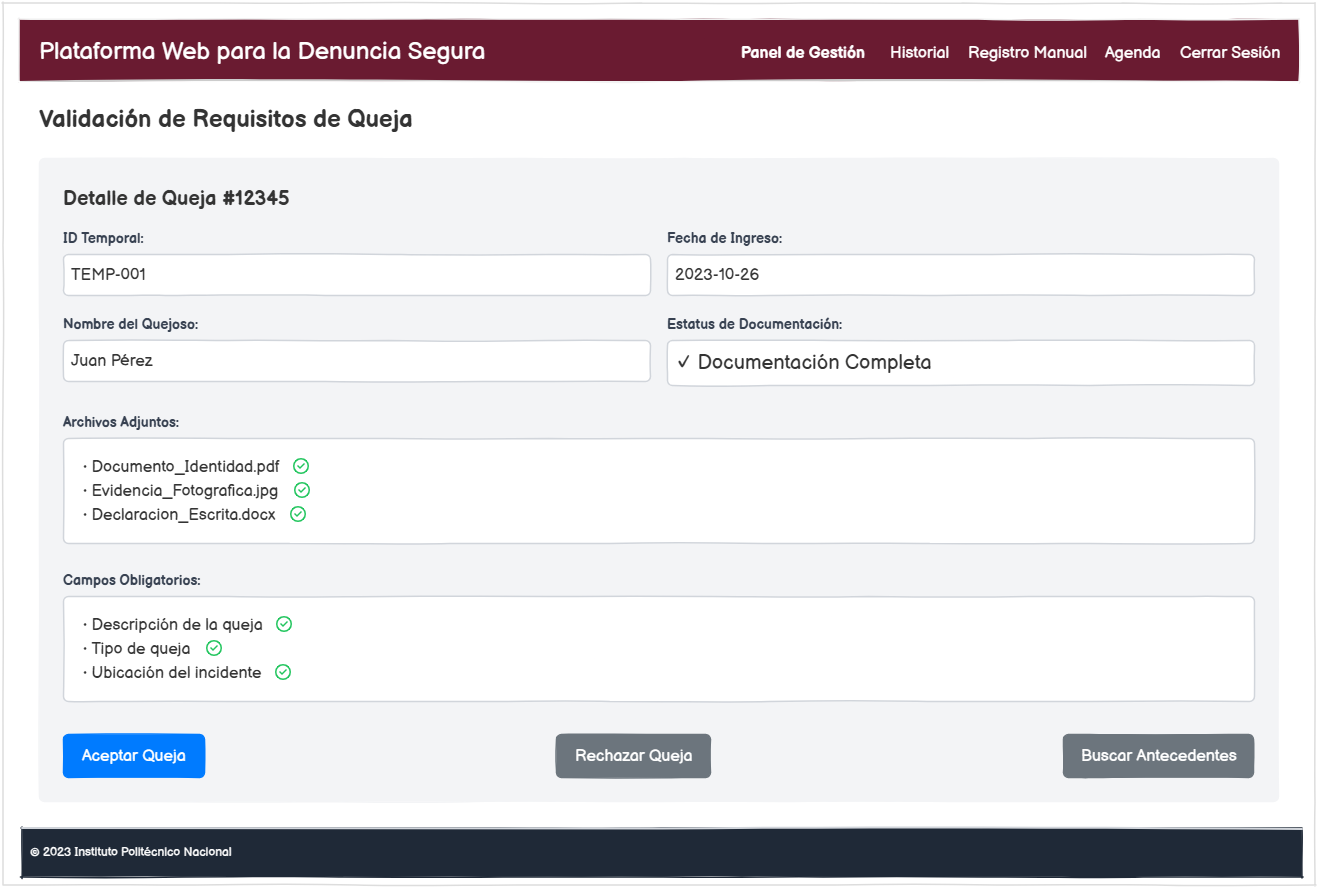
\includegraphics[width=0.85\textwidth]{imagenes/recepcion/ValidaciónRequisitosQueja.png}
    \caption{MA-05: Módulo de validación de requisitos de queja.}
    \label{fig:ma05_validacion_requisitos}
\end{figure}

\noindent \textbf{Descripción de la interfaz (MA-05):} \\
Esta interfaz constituye el control de calidad del sistema, permitiendo al personal de recepción asegurar que cada solicitud cumpla con los estándares normativos antes de su proceso. Los elementos operativos son:
\begin{itemize}
    \item \textbf{Resumen del Expediente Temporal:} Muestra los datos básicos del registro (ID temporal, fecha de ingreso y nombre) para contextualizar la revisión.
    \item \textbf{Estatus de Documentación:} Un campo de confirmación visual que indica si el paquete informativo está completo o requiere ajustes.
    \item \textbf{Checklist de Archivos Adjuntos:} Un panel detallado que lista los documentos digitales recibidos (PDF, imágenes, Word). El sistema marca con iconos de verificación verdes aquellos archivos que han sido cargados exitosamente.
    \item \textbf{Validación de Campos Obligatorios:} Verifica que la descripción, tipo de queja y ubicación del incidente hayan sido capturados correctamente, garantizando que el expediente no tenga vacíos de información.
    \item \textbf{Acciones de Dictaminación:} Tres botones de control que definen el destino de la queja: "Aceptar Queja" para formalizarla, "Rechazar Queja" para devolverla al usuario, o "Buscar Antecedentes" para una revisión histórica previa a la canalización.
\end{itemize}

\vspace{1cm}

% --- VISTA 06: NOTIFICACIÓN DE RECHAZO ---
\begin{figure}[h]
    \centering
    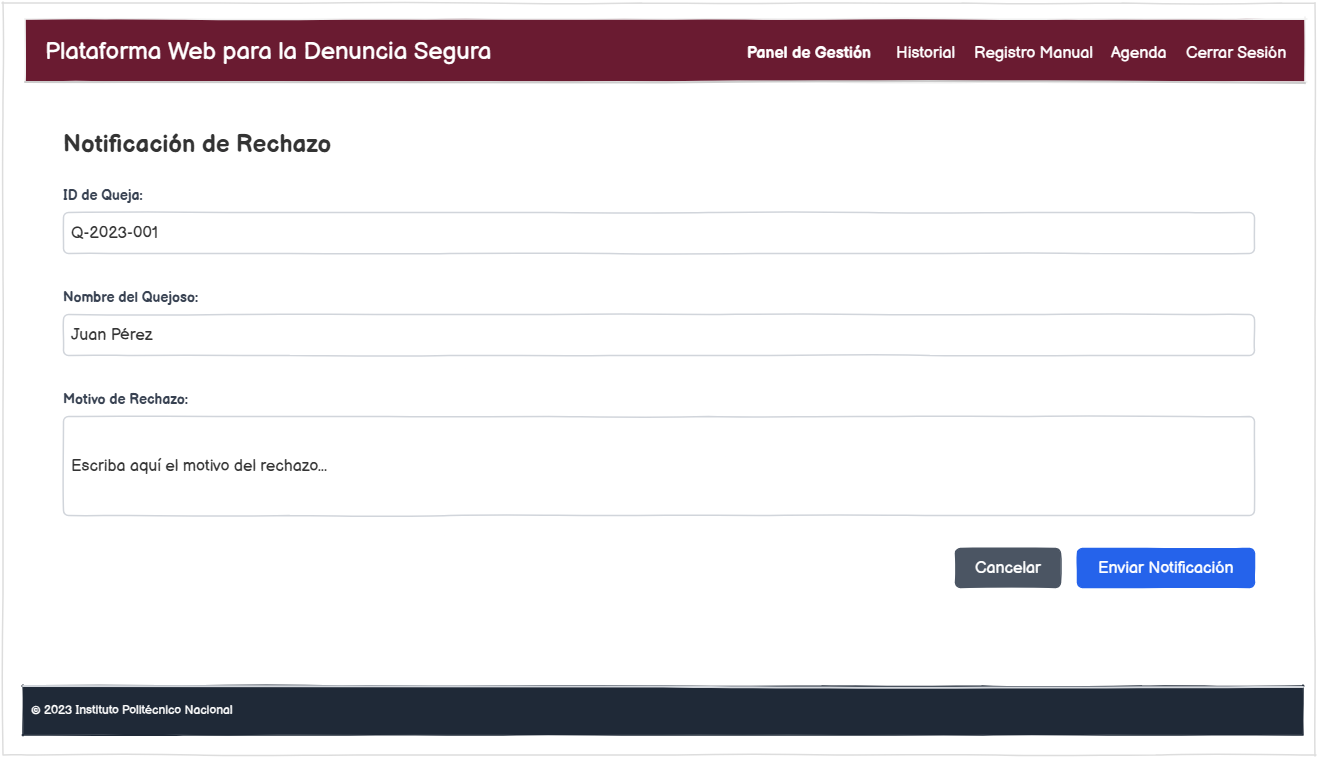
\includegraphics[width=0.85\textwidth]{imagenes/recepcion/NotificacionRechazo.png}
    \caption{MA-06: Interfaz de notificación de rechazo por incumplimiento.}
    \label{fig:ma06_notificacion_rechazo}
\end{figure}

\noindent \textbf{Descripción de la interfaz (MA-06):} \\
Esta pantalla se activa cuando el personal de recepción determina que la solicitud no cumple con los requisitos mínimos para ser procesada. Su función es informar al quejoso de manera formal y clara sobre las deficiencias detectadas. Los componentes son:
\begin{itemize}
    \item \textbf{Identificación del Trámite:} Campos de solo lectura que muestran el ID de la Queja y el nombre del quejoso, asegurando que la notificación esté correctamente vinculada al expediente en cuestión.
    \item \textbf{Cuerpo del Motivo de Rechazo:} Área de texto de formato libre donde el administrativo debe redactar de forma detallada la razón técnica o jurídica del rechazo (ej. falta de pruebas, datos inconsistentes o falta de firmas).
    \item \textbf{Acciones de Comunicación:} Botón de "Enviar Notificación" que dispara un correo electrónico automático al usuario con el texto redactado, y un botón de "Cancelar" para regresar al módulo de validación sin realizar cambios.
    \item \textbf{Consistencia en la Navegación:} El menú superior permite al personal desplazarse hacia otras tareas administrativas como la Agenda o el Historial una vez concluida la acción de rechazo.
\end{itemize}

\vspace{1cm}

% --- VISTA 07: ANTECEDENTES Y CANALIZACIÓN ---
\begin{figure}[h]
    \centering
    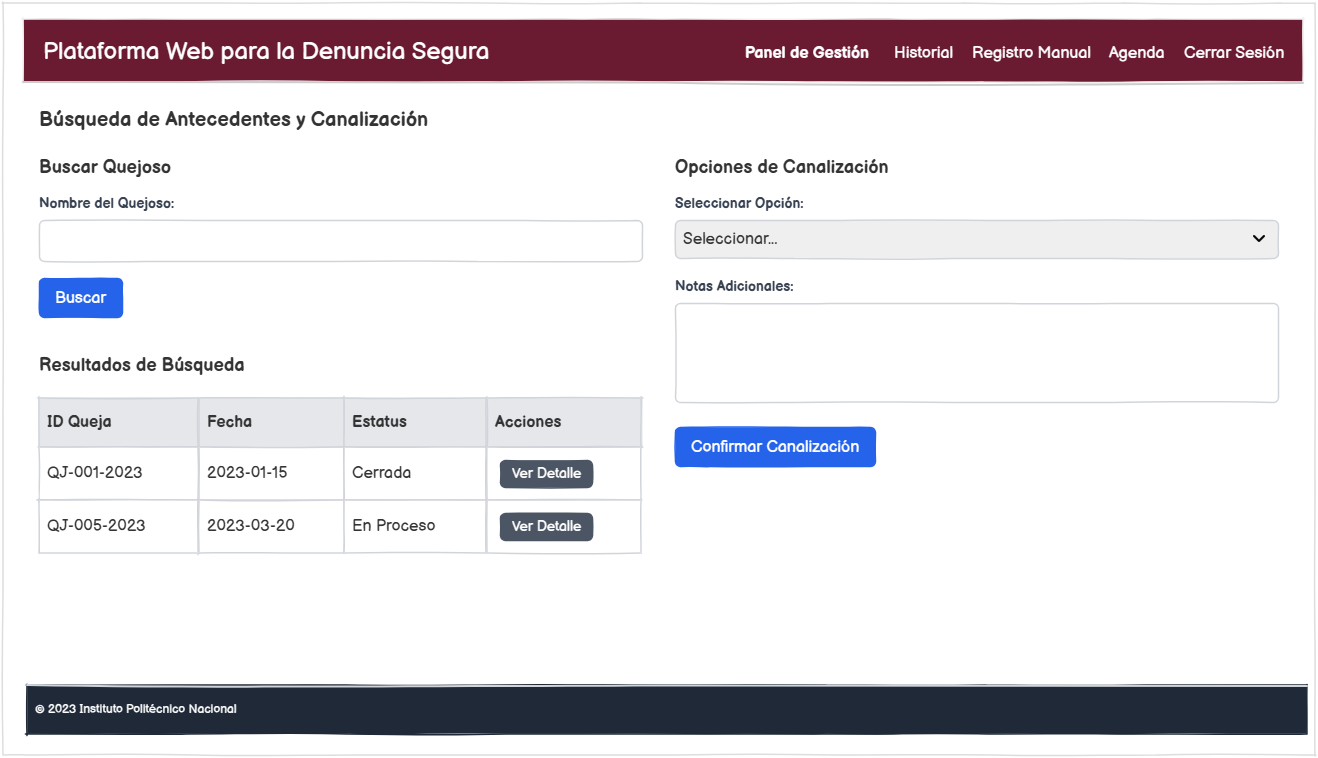
\includegraphics[width=0.85\textwidth]{imagenes/recepcion/BuesquedaAntecedentesCanalizacion.png}
    \caption{MA-07: Módulo de búsqueda de antecedentes y canalización interna.}
    \label{fig:ma07_canalizacion}
\end{figure}

\noindent \textbf{Descripción de la interfaz (MA-07):} \\
Esta pantalla representa el último paso operativo en el área de Recepción. Su objetivo es doble: verificar si el quejoso tiene procesos previos y formalizar el traslado del expediente al siguiente departamento. Sus componentes son:
\begin{itemize}
    \item \textbf{Búsqueda de Antecedentes:} Un motor de búsqueda por nombre que permite identificar si el usuario ha presentado quejas anteriormente. Esto evita la duplicidad de folios y permite al personal administrativo conocer el historial del solicitante.
    \item \textbf{Tabla de Resultados:} Despliega las quejas previas encontradas, mostrando su ID, fecha de registro y estatus actual (ej. Cerrada, En Proceso), con la opción de "Ver Detalle" para cada una.
    \item \textbf{Opciones de Canalización:} Panel derecho donde el personal selecciona mediante un menú desplegable el área de destino (en este flujo, Primer Contacto). 
    \item \textbf{Notas Adicionales:} Área de texto para incluir observaciones relevantes que el siguiente departamento deba conocer antes de tomar el caso.
    \item \textbf{Confirmación de Envío:} El botón "Confirmar Canalización" formaliza la salida del expediente del área de Recepción, actualizando su estatus en el flujo de trabajo global.
\end{itemize}

\subsection{Departamento de Primer Contacto}
Este departamento se encarga de la atención personalizada al quejoso. Su función principal es realizar la entrevista inicial, analizar la naturaleza de la queja y determinar si el asunto es competencia de la Defensoría o si debe ser orientado a otra instancia.

% --- VISTA 08: BANDEJA DE ANÁLISIS ---
\begin{figure}[h]
    \centering
    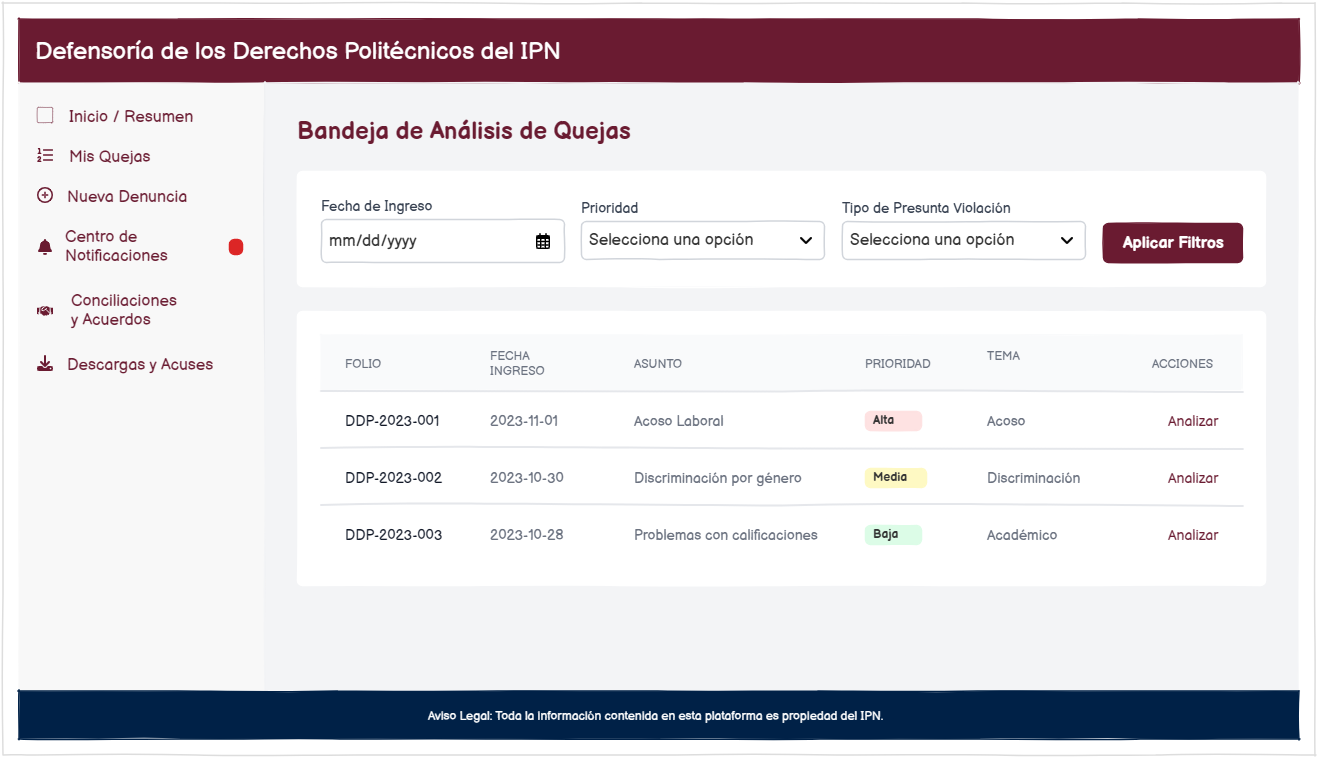
\includegraphics[width=0.85\textwidth]{imagenes/primercontacto/DashboardoAnalisisQuejas.png}
    \caption{MA-08: Bandeja de análisis de quejas para Primer Contacto.}
    \label{fig:ma08_analisis_dashboard}
\end{figure}

\noindent \textbf{Descripción de la interfaz (MA-08):} \\
Esta interfaz es la herramienta principal del abogado o analista de Primer Contacto. Su función es organizar las quejas canalizadas desde Recepción para iniciar el estudio de fondo. Los elementos clave son:
\begin{itemize}
    \item \textbf{Módulo de Filtrado Avanzado:} Permite segmentar la carga de trabajo por fecha de ingreso, nivel de prioridad y tipo de presunta violación (académica, de género, laboral, etc.), facilitando la atención de casos urgentes.
    \item \textbf{Tabla de Gestión Operativa:} Despliega los expedientes con el Folio oficial (ej. DDP-2023-XXX). Incluye columnas para identificar el asunto y el tema asignado automáticamente o por recepción.
    \item \textbf{Etiquetas de Prioridad:} Sistema visual de colores (rojo para Alta, amarillo para Media, verde para Baja) que permite una rápida jerarquización de los casos según la gravedad de los hechos reportados.
    \item \textbf{Acción de Análisis:} El control "Analizar" dirige al funcionario al expediente detallado para comenzar la calificación jurídica y la preparación de la entrevista inicial.
\end{itemize}

\vspace{1cm}

\begin{figure}[h]
    \centering
    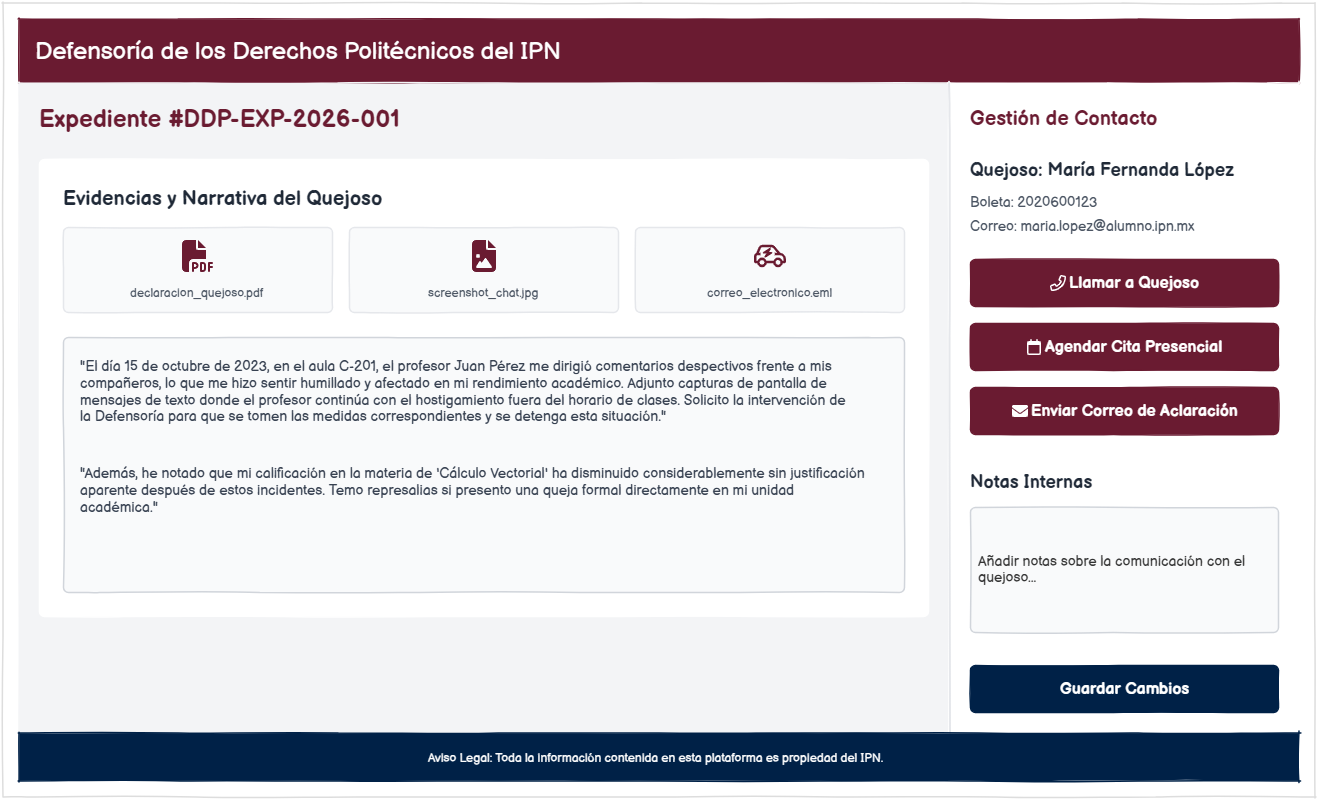
\includegraphics[width=0.85\textwidth]{imagenes/primercontacto/AnalisisExpediente.png}
    \caption{MA-09: Interfaz de estudio de narrativa y evidencias.}
    \label{fig:ma09_analisis_expediente}
\end{figure}

\noindent \textbf{Descripción de la interfaz (MA-09):} \\
Esta pantalla centraliza toda la información aportada por el quejoso para su evaluación legal. Sus componentes son:
\begin{itemize}
    \item \textbf{Visor de Evidencias:} Acceso directo a archivos adjuntos con iconos diferenciados por formato (PDF, JPG, EML).
    \item \textbf{Narrativa del Quejoso:} Área de lectura de los hechos para la identificación de puntos clave y presuntas violaciones de derechos.
    \item \textbf{Panel de Gestión de Contacto:} Herramientas para la comunicación inmediata (Llamar, Agendar o Enviar Correo) que permiten solicitar aclaraciones necesarias para el dictamen.
    \item \textbf{Bitácora de Notas Internas:} Campo para observaciones técnicas del analista que facilitan la continuidad del caso.
\end{itemize}

% --- VISTA 10: AGENDAR CITAS ---
\begin{figure}[h]
    \centering
    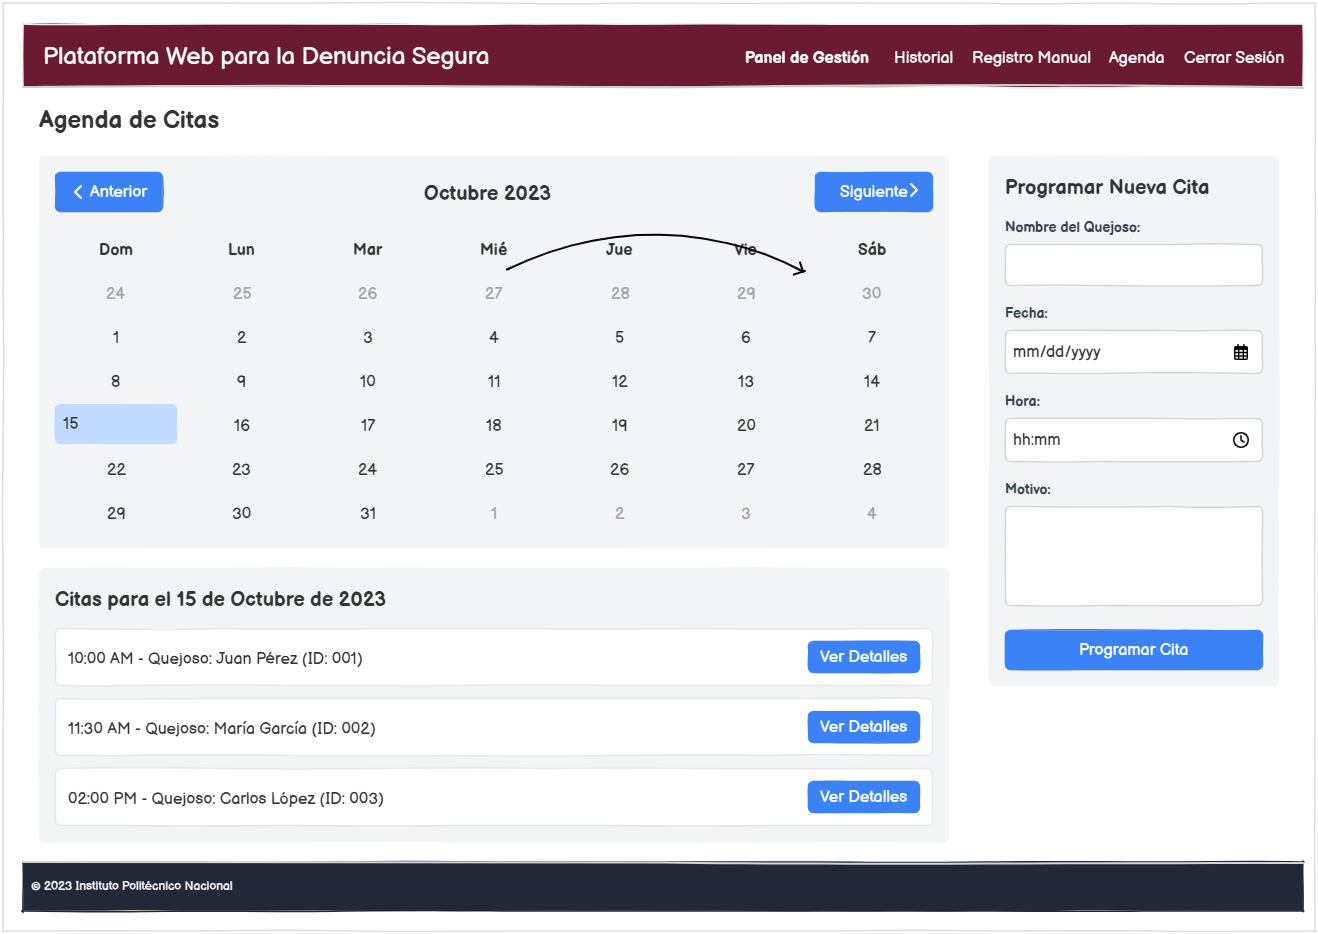
\includegraphics[width=0.85\textwidth]{imagenes/primercontacto/AgendarCitas.png}
    \caption{MA-10: Módulo de agenda institucional para entrevistas de calificación.}
    \label{fig:ma10_agenda_citas}
\end{figure}

\noindent \textbf{Descripción de la interfaz (MA-10):} \\
Esta interfaz es fundamental para la interacción directa entre el analista y el quejoso. Permite organizar las diligencias necesarias para profundizar en los hechos reportados:
\begin{itemize}
    \item \textbf{Calendario de Disponibilidad:} Un visor dinámico que muestra las citas programadas por el personal de Primer Contacto, evitando el traslape de horarios y optimizando el uso de las salas de entrevista.
    \item \textbf{Formulario de Registro de Cita:} Panel lateral para capturar los detalles de la nueva reunión, vinculando automáticamente el ID del Quejoso con una fecha, hora y modalidad (presencial o virtual).
    \item \textbf{Lista de Próximas Entrevistas:} Un listado rápido al pie del formulario que permite identificar las citas más cercanas, facilitando la preparación previa del expediente por parte del abogado encargado.
    \item \textbf{Sincronización de Estatus:} Al agendar una cita, el sistema actualiza el estatus del expediente a 'En Entrevista', notificando automáticamente al usuario a través del portal del quejoso.
\end{itemize}

\clearpage %

\begin{figure}[h]
    \centering
    % Se quitó la extensión para que LaTeX busque automáticamente el archivo disponible
    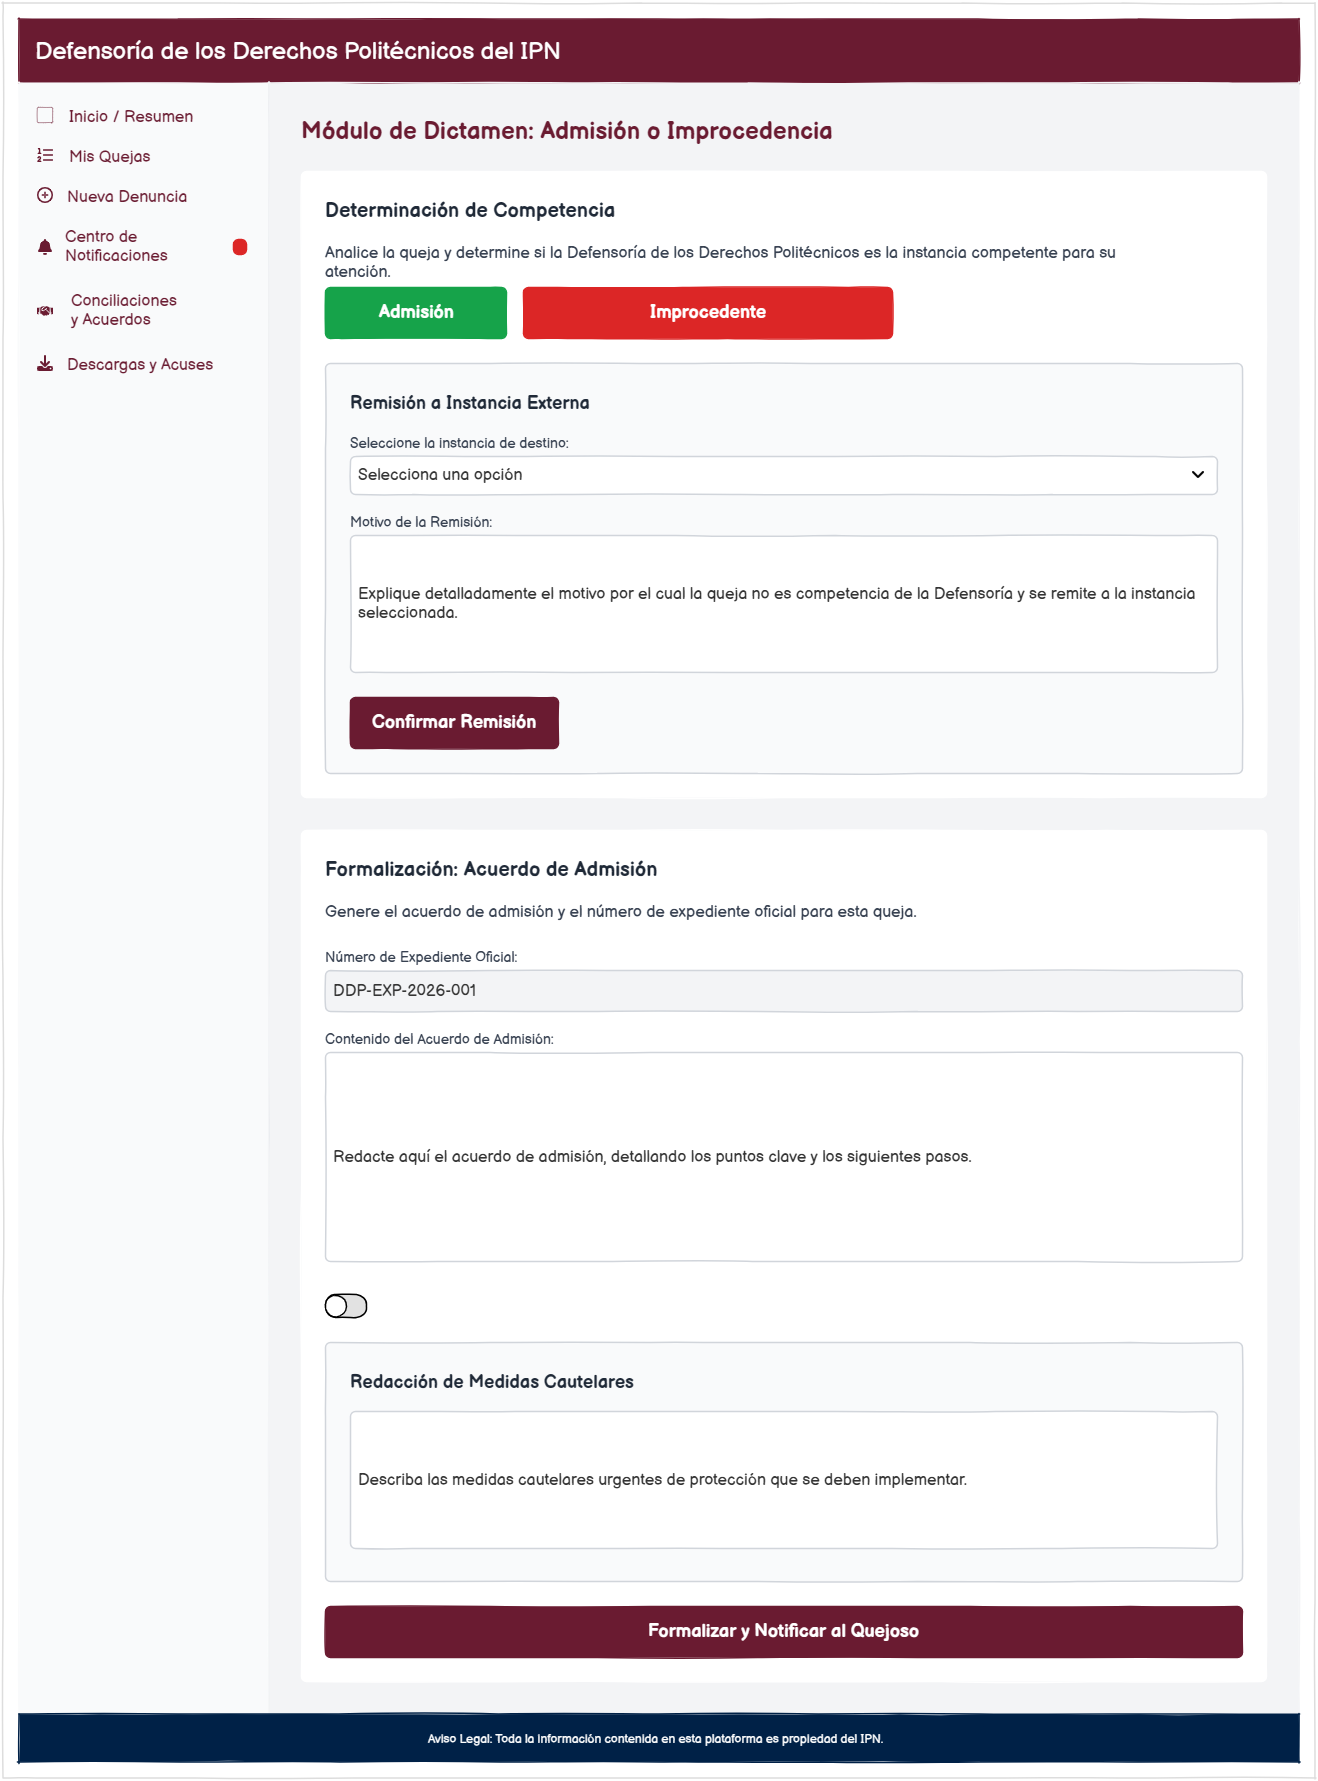
\includegraphics[width=0.85\textwidth]{imagenes/primercontacto/DictamenCompetencia}
    \caption{MA-11: Módulo de dictamen de admisión o improcedencia.}
    \label{fig:ma11_dictamen_competencia}
\end{figure}
\clearpage %

\noindent \textbf{Descripción de la interfaz (MA-11):} \\
Esta es la pantalla de resolución técnica del departamento de Primer Contacto. Representa el acto jurídico donde se decide el curso legal de la queja:
\begin{itemize}
    \item \textbf{Determinación de Competencia:} Botones de selección de alto contraste para definir la procedencia del caso (Admisión o Improcedencia).
    \item \textbf{Gestión de Improcedencia:} En caso de no ser competencia de la Defensoría, se habilita una sección para seleccionar la instancia externa de remisión y redactar los motivos legales de dicha decisión.
    \item \textbf{Acuerdo de Admisión:} Si el caso es admitido, el sistema genera el número de expediente oficial y ofrece un área para redactar los puntos clave del acuerdo.
    \item \textbf{Medidas Cautelares:} Incluye un control conmutador para activar la redacción de medidas urgentes de protección que deban implementarse inmediatamente para salvaguardar la integridad del quejoso.
    \item \textbf{Formalización:} El botón final procesa el dictamen y notifica automáticamente al usuario sobre la admisión o el curso que seguirá su trámite.
\end{itemize}

\clearpage %


% --- VISTA 12: FINALIZACIÓN Y NOTIFICACIÓN ---
\begin{figure}[h]
    \centering
    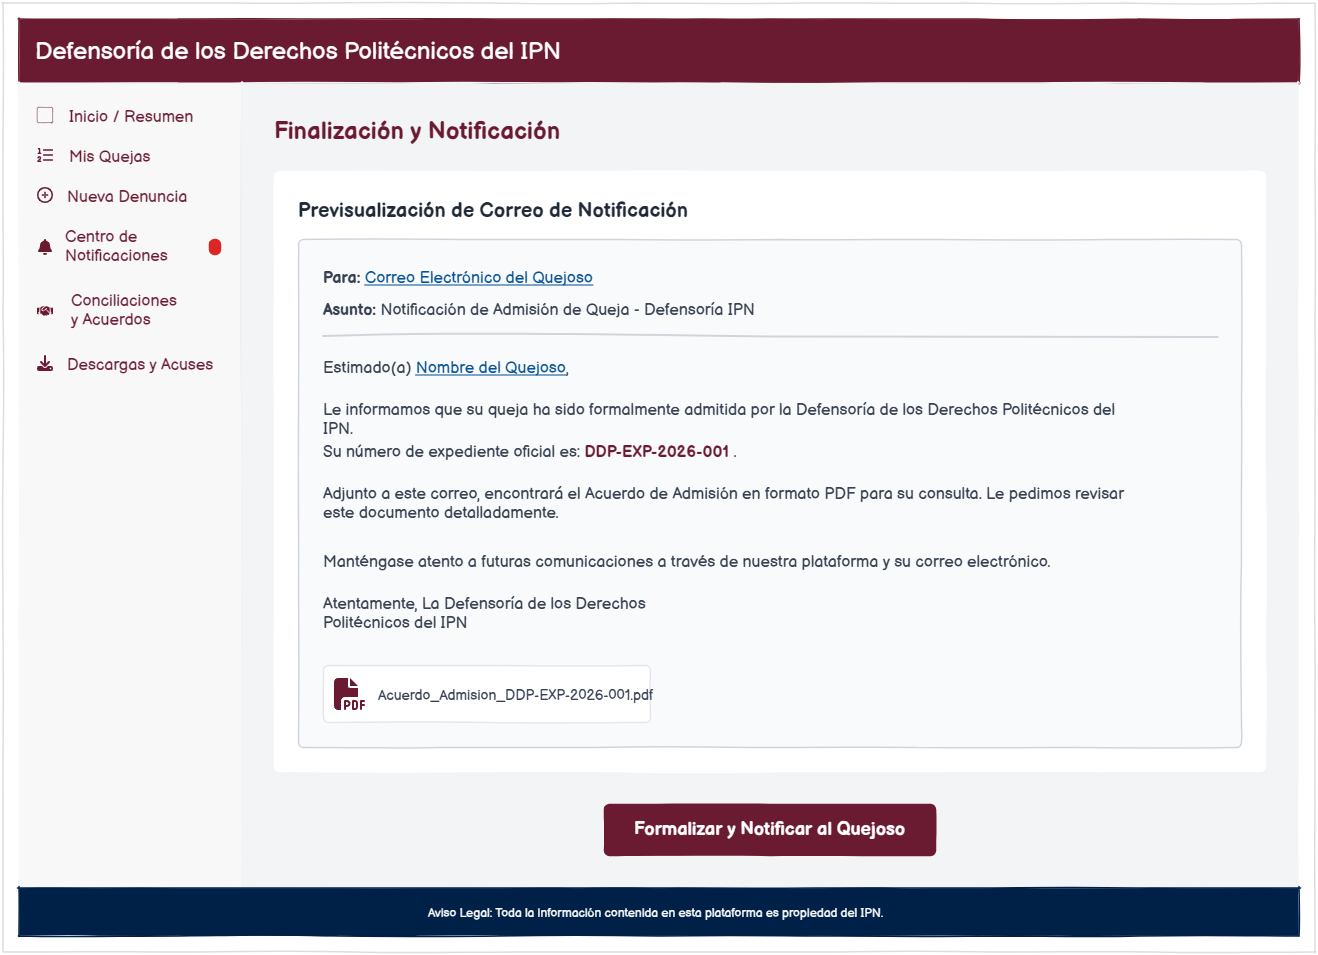
\includegraphics[width=0.85\textwidth]{imagenes/primercontacto/FormalizacionNotificacion.png}
    \caption{MA-12: Interfaz de previsualización y notificación de admisión oficial.}
    \label{fig:ma12_finalizacion_notificacion}
\end{figure}

\noindent \textbf{Descripción de la interfaz (MA-12):} \\
Esta pantalla constituye el paso final del departamento de Primer Contacto antes de trasladar el expediente al área de instrucción (Subdefensoría). Su propósito es garantizar la transparencia mediante la notificación automática al quejoso:
\begin{itemize}
    \item \textbf{Previsualización de Notificación:} Presenta el cuerpo del correo electrónico que será enviado, permitiendo al analista verificar que los datos del quejoso y el número de expediente oficial (ej. DDP-EXP-2026-001) sean correctos.
    \item \textbf{Gestión de Documentos Adjuntos:} Muestra el archivo PDF del "Acuerdo de Admisión" generado en el paso anterior, el cual queda vinculado permanentemente al correo y al repositorio del expediente.
    \item \textbf{Acción de Formalización:} El botón "Formalizar y Notificar al Quejoso" ejecuta tres acciones simultáneas en el sistema: actualiza el estatus de la queja a "Admitida", realiza el envío masivo de la notificación y habilita el acceso del expediente al departamento de Subdefensoría.
    \item \textbf{Entorno de Gestión:} Mantiene la barra lateral de navegación administrativa, permitiendo al personal confirmar que existen notificaciones pendientes en otros casos mientras concluye el actual.
\end{itemize}

\end{appendices}